\documentclass[11pt,a4paper]{article}

% ----------------- Packages -----------------
\usepackage[margin=1in]{geometry}
\usepackage{amsmath, amssymb, amsfonts, bm, mathtools}
\usepackage{siunitx}
\usepackage{graphicx}
\usepackage{booktabs}
\usepackage[dvipsnames]{xcolor}
\usepackage{hyperref}
\usepackage[nameinlink,capitalise]{cleveref}
\usepackage{enumitem}
\usepackage{caption}
\usepackage{float}
\usepackage{listings}
\usepackage{tabularx}
\usepackage{multirow}

\hypersetup{
  colorlinks=true,
  urlcolor=MidnightBlue,
  linkcolor=MidnightBlue,
  citecolor=MidnightBlue
}

% ----------------- Listings (Python) -----------------
\lstdefinestyle{mystyle}{
  language=Python,
  basicstyle=\ttfamily\small,
  keywordstyle=\color{MidnightBlue}\bfseries,
  stringstyle=\color{OliveGreen},
  commentstyle=\color{Gray},
  showstringspaces=false,
  frame=single,
  rulecolor=\color{Gray},
  numbers=left,
  numberstyle=\tiny\color{Gray},
  breaklines=true,
  tabsize=2,
  captionpos=b
}
\lstset{style=mystyle}

% ----------------- Math helpers -----------------
\DeclareMathOperator{\E}{\mathbb{E}}
\DeclareMathOperator{\Var}{\mathbb{V}ar}
\DeclareMathOperator{\Cov}{\mathbb{C}ov}
\DeclareMathOperator{\corr}{corr}
\newcommand{\1}{\mathbf{1}}
\newcommand{\vect}[1]{\bm{#1}}

% ----- Caminho dos gráficos (use barras / no Windows) -----
% Dica: use barras normais e preserve espaços (LaTeX aceita dentro de { }).
\graphicspath{{C:/Users/Lenovo/Desktop/Desktop/Mestrado FGV/RiskFrontier/}}

\title{Risk Frontier para Carteiras de Crédito Consignado (INSS)\\
\large Estrutura metodológica, equações, script e exemplos de entrada/saída}
\author{}
\date{\today}

\begin{document}
\maketitle

\section{Visão geral}
O objetivo é construir uma \emph{fronteira eficiente} de risco--retorno para carteiras agregadas por grupos homogêneos de risco (GHRs), levando em conta: dinâmica de inadimplência via roll-rates, EL/UL/EC (Vasicek/IRB), ajuste de maturidade, \emph{carry cost} e normalização por prazo (\emph{EAA}). O script gera a fronteira e classifica GHRs em eficientes/ineficientes. Há três visões: \textbf{Total}, \textbf{Sem Safra} e \textbf{Só Safra}.

\section{Fluxos e saldo (Price)}
Para um contrato com valor liberado $V$, taxa mensal $i$ e prazo $N$:
\[
\mathrm{PMT}=V\frac{i(1+i)^N}{(1+i)^N-1},\quad
\mathrm{Saldo}(n)=V(1+i)^n-\mathrm{PMT}\frac{(1+i)^n-1}{i}.
\]

\section{Roll-rates e PD condicional}
Com buckets $\{\text{current},30,60,90,\text{wo}\}$ e matriz mensal $\mathbf{P}$ (wo absorvente), a prob. acumulada de default em $H$ meses:
\[
p_{\text{def}}(H)=\sum_{t=1}^{H}\vect{s}_{t-1}\mathbf{P}\,\vect{e}_{\text{wo}},\quad
\vect{s}_t=\vect{s}_{t-1}\mathbf{P},\ \ s_t(\text{wo})\gets 0.
\]
LGD por bucket vem de tabela; EL forward usa $p_{\text{def}}(H)\cdot \text{LGD}\cdot \text{EAD}$.

\section{Carry cost}
Com funding $k_f$ a.a. e spread $s$ a.a., taxas mensais $k_f^{(m)}$ e $s^{(m)}$. Se suspende accrual em atraso:
\[
\mathrm{Carry}(H)=H\cdot\big(k_f^{(m)}\cdot \text{EAD} + \1_{\text{atraso}}\cdot s^{(m)}\cdot \text{EAD} + \mathrm{OPEX}(\text{bucket})\big).
\]

\section{EL, UL, EC e ajuste de maturidade}
\[
\mathrm{EL}=PD\cdot LGD\cdot EAD,\quad
\mathrm{UL}=LGD\cdot EAD\cdot \Phi\!\left(\frac{\Phi^{-1}(PD)+\sqrt{\rho}\,z_\alpha}{\sqrt{1-\rho}}\right),
\]
\[
EC_{1y}=\max(\mathrm{UL}-\mathrm{EL},0),\quad
EC=EC_{1y}\cdot \mathrm{MA}(M),\ \ \mathrm{MA}(M)=\frac{1+(M-2.5)b}{1-1.5b}.
\]

\section{Normalização por prazo (EAA)}
Com prazo médio remanescente $M$ (anos) e taxa $K$:
\[
\mathrm{NPV}_{\text{proxy}}\approx \mathrm{Retorno\ Anual}\cdot M,\qquad
\mathrm{EAA}=\mathrm{NPV}_{\text{proxy}}\cdot \frac{K}{1-(1+K)^{-M}}.
\]

\section{Fronteira eficiente}
Amostra-se $\vect{w}$ (Dirichlet), calcula-se o par $(EC(\vect{w}),R(\vect{w}))$ e toma-se a envoltória superior por janelas de $EC$. Para cada GHR $i$: $\eta_i=\frac{R_i}{\widehat{R}(EC_i)}$ e $\mathrm{ROE}_i=\frac{R_i}{EC_i}$.

% ============================================================
\section{Exemplo de dados de entrada}
\label{sec:exemplo-entrada}
Os arquivos de entrada são três abas principais: \texttt{contratos}, \texttt{ghr\_param}, \texttt{params}. Abaixo, \emph{amostras reduzidas} (somente para referência visual).

\subsection*{Aba \texttt{contratos} (exemplo)}
\begin{table}[H]\centering
\small
\begin{tabular}{lcccccccc}
\toprule
ContratoID & GHR & Estado & Valor\_Liberado & Prazo\_Meses & Meses\_Pagos & Saldo\_Atual & Bucket\_Atraso & DPD \\
\midrule
1001 & GHR\_1 & Em dia   & 8{,}500.00 & 72 & 15 & 7{,}420.10 & current & 0 \\
1002 & GHR\_2 & Em atraso& 12{,}000.00 & 60 & 24 & 9{,}815.32 & 30      & 18 \\
1003 & GHR\_3 & Na Safra & 9{,}000.00 & 84 & 0  & 9{,}000.00 & current & 0 \\
1004 & GHR\_4 & Em dia   & 15{,}500.00 & 48 & 10 & 12{,}870.25& current & 0 \\
1005 & GHR\_5 & Em atraso& 6{,}800.00  & 36 & 20 & 4{,}210.77 & 60      & 45 \\
\bottomrule
\end{tabular}
\caption{Amostra ilustrativa de \texttt{contratos}. Colunas adicionais opcionais: \texttt{Overs\_Flag}, \texttt{IsDelayed\_Flag}.}
\end{table}

\subsection*{Aba \texttt{ghr\_param} (exemplo)}
\begin{table}[H]\centering
\small
\begin{tabular}{lccc}
\toprule
GHR & PD\_Base (a.a.) & LGD\_Base & Spread\_aa \\
\midrule
GHR\_1 & 0.015 & 0.18 & 0.14 \\
GHR\_2 & 0.020 & 0.22 & 0.16 \\
GHR\_3 & 0.030 & 0.25 & 0.18 \\
GHR\_4 & 0.050 & 0.28 & 0.20 \\
GHR\_5 & 0.080 & 0.30 & 0.22 \\
\bottomrule
\end{tabular}
\caption{Parâmetros médios por GHR.}
\end{table}

\subsection*{Aba \texttt{params} (exemplo)}
\begin{table}[H]\centering
\small
\begin{tabular}{lc}
\toprule
Parametro & Valor \\
\midrule
Funding\_aa & 0.10 \\
H\_fwd\_meses & 12 \\
Modo\_prazo & eaa \\
K\_EAA & 0.12 \\
\bottomrule
\end{tabular}
\caption{Parâmetros globais (opcional).}
\end{table}

\subsection*{Opcionais: \texttt{roll\_rates}, \texttt{prov\_reg}, \texttt{lgd\_bucket}}
\begin{table}[H]\centering
\small
\begin{tabular}{lccccc}
\toprule
 & current & 30 & 60 & 90 & wo \\
\midrule
current & 0.92 & 0.06 & 0.01 & 0.00 & 0.01 \\
30      & 0.35 & 0.45 & 0.15 & 0.02 & 0.03 \\
60      & 0.10 & 0.25 & 0.45 & 0.15 & 0.05 \\
90      & 0.02 & 0.05 & 0.28 & 0.45 & 0.20 \\
wo      & 0.00 & 0.00 & 0.00 & 0.00 & 1.00 \\
\bottomrule
\end{tabular}
\caption{Exemplo de matriz \texttt{roll\_rates} mensal (linhas normalizadas).}
\end{table}

\begin{table}[H]\centering
\small
\begin{tabular}{lcc}
\toprule
bucket & prov\_reg (pct EAD) & lgd \\
\midrule
current & 0.02 & 0.25 \\
30      & 0.10 & 0.30 \\
60      & 0.30 & 0.35 \\
90      & 0.50 & 0.40 \\
wo      & 1.00 & 0.45 \\
\bottomrule
\end{tabular}
\caption{Exemplo de provisão regulatória e LGD por bucket.}
\end{table}

% ============================================================
\section{Resultados gráficos (arquivos gerados)}
\label{sec:resultados}
Os gráficos abaixo são lidos de \texttt{C:/Users/Lenovo/Desktop/Desktop/Mestrado FGV/RiskFrontier/}, onde o script salva os PNGs. Se necessário, ajuste o caminho em \verb|\graphicspath| no preâmbulo.

\subsection*{Visão Total}
\begin{figure}[H]\centering
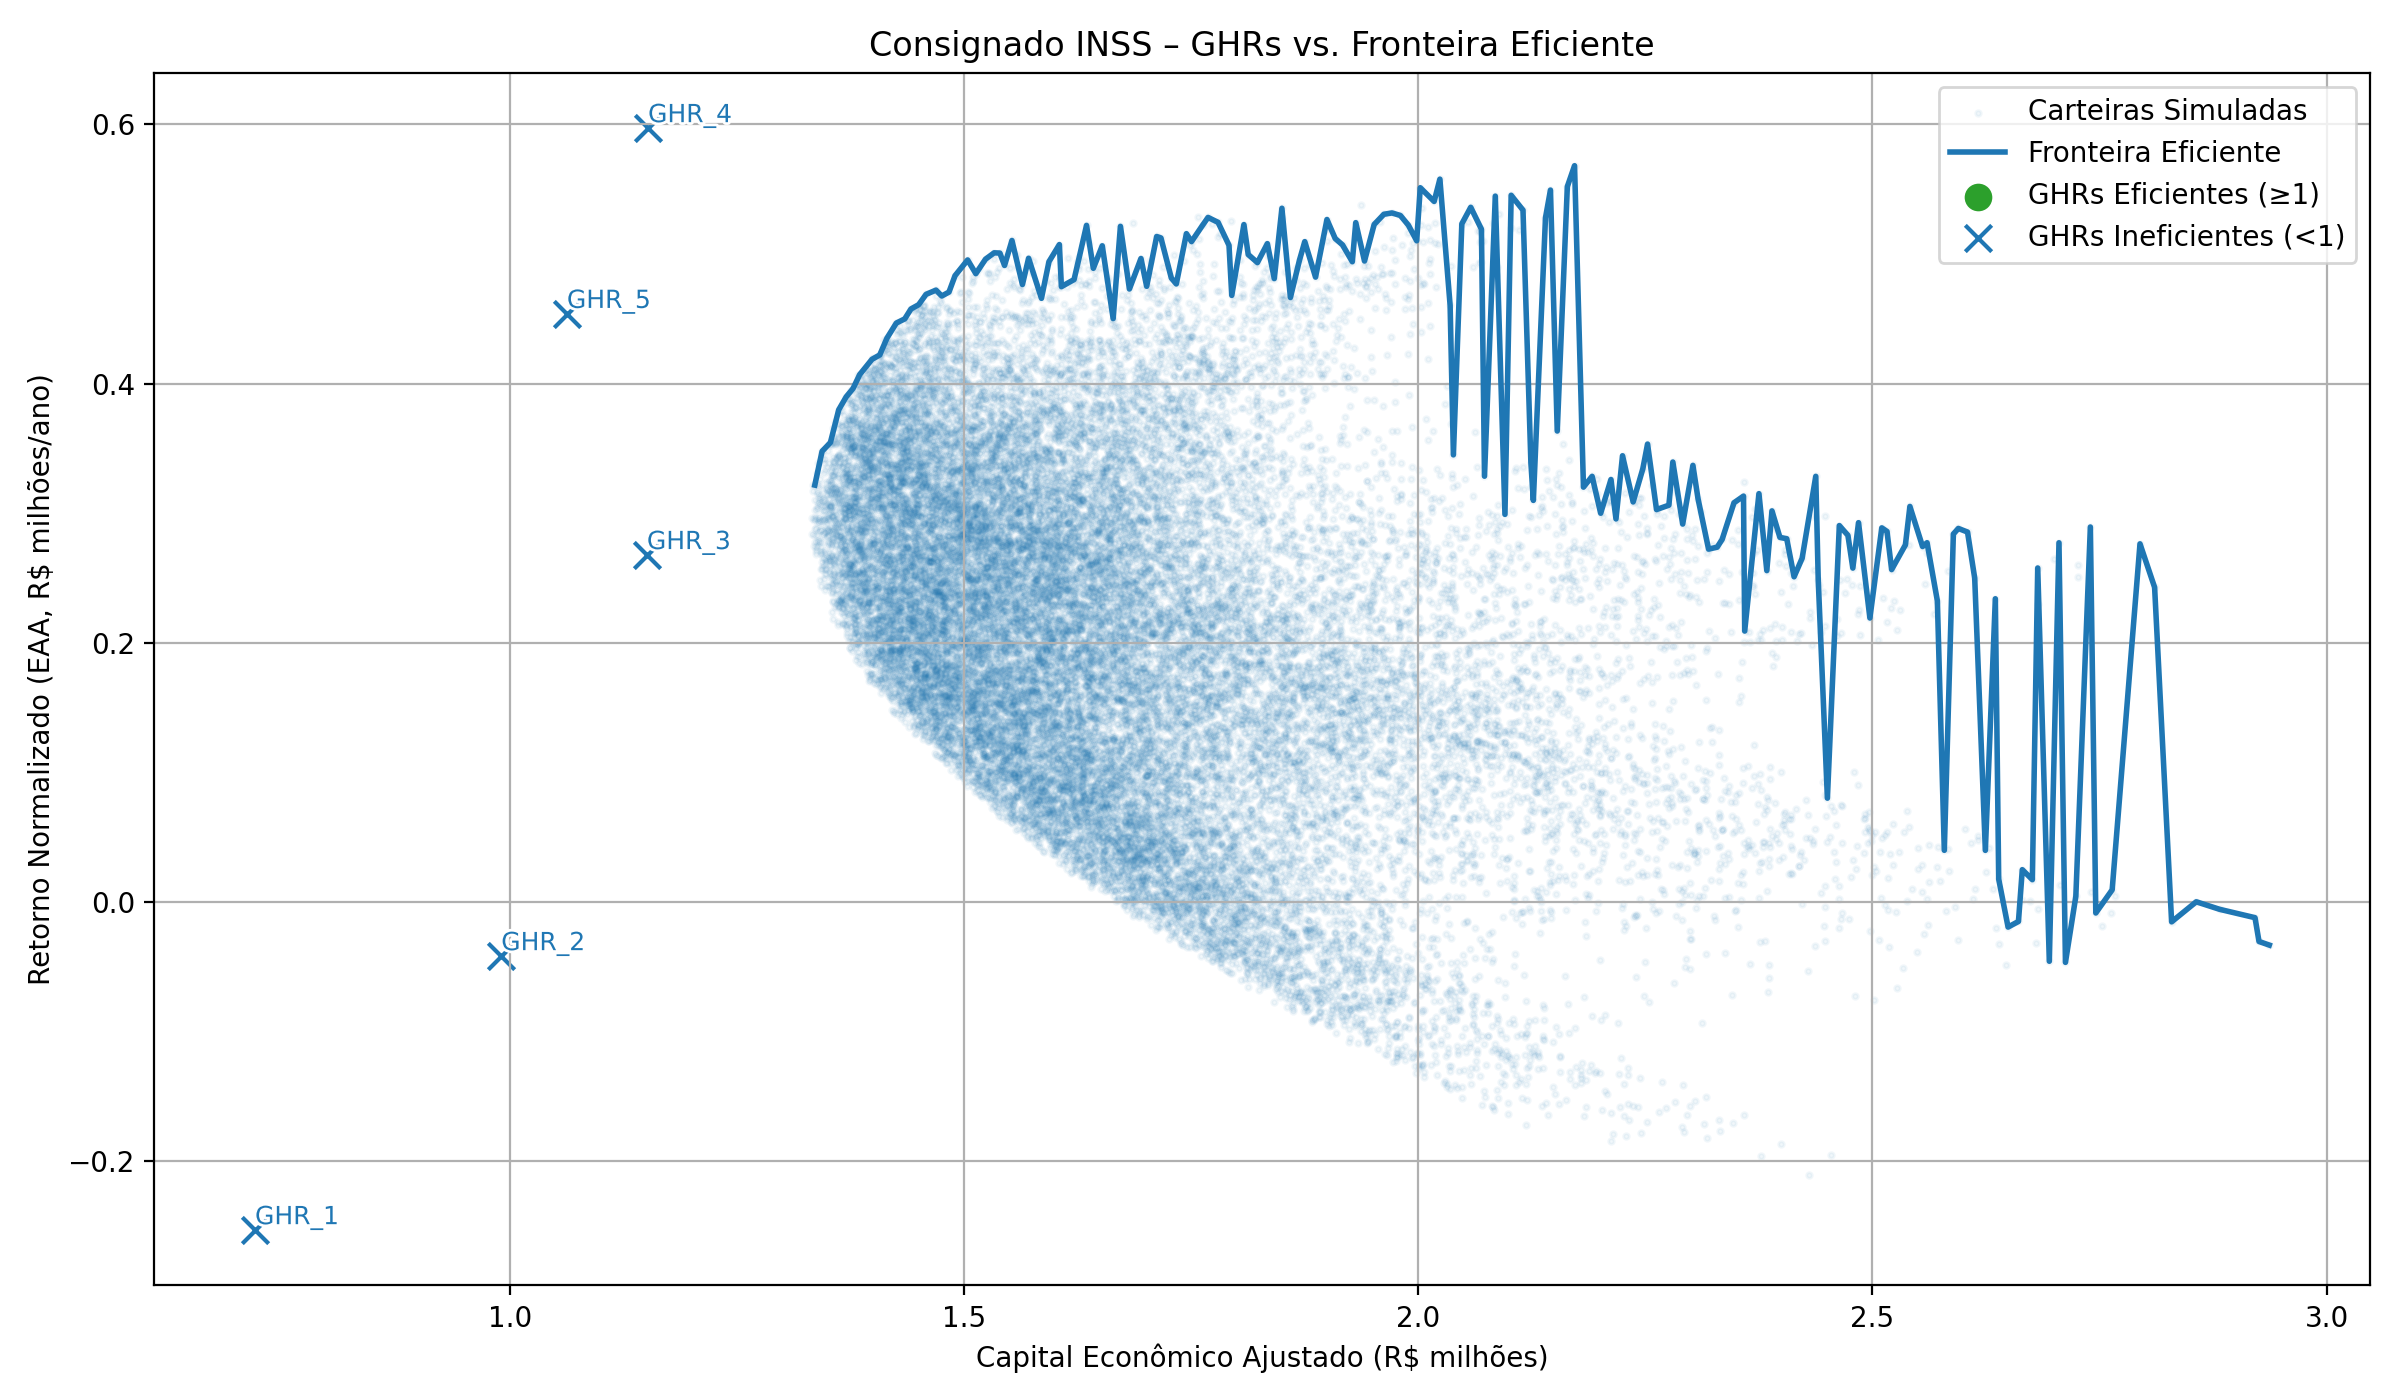
\includegraphics[width=.85\linewidth]{fronteira.png}
\caption{Fronteira eficiente – Visão Total.}
\end{figure}

\begin{figure}[H]\centering
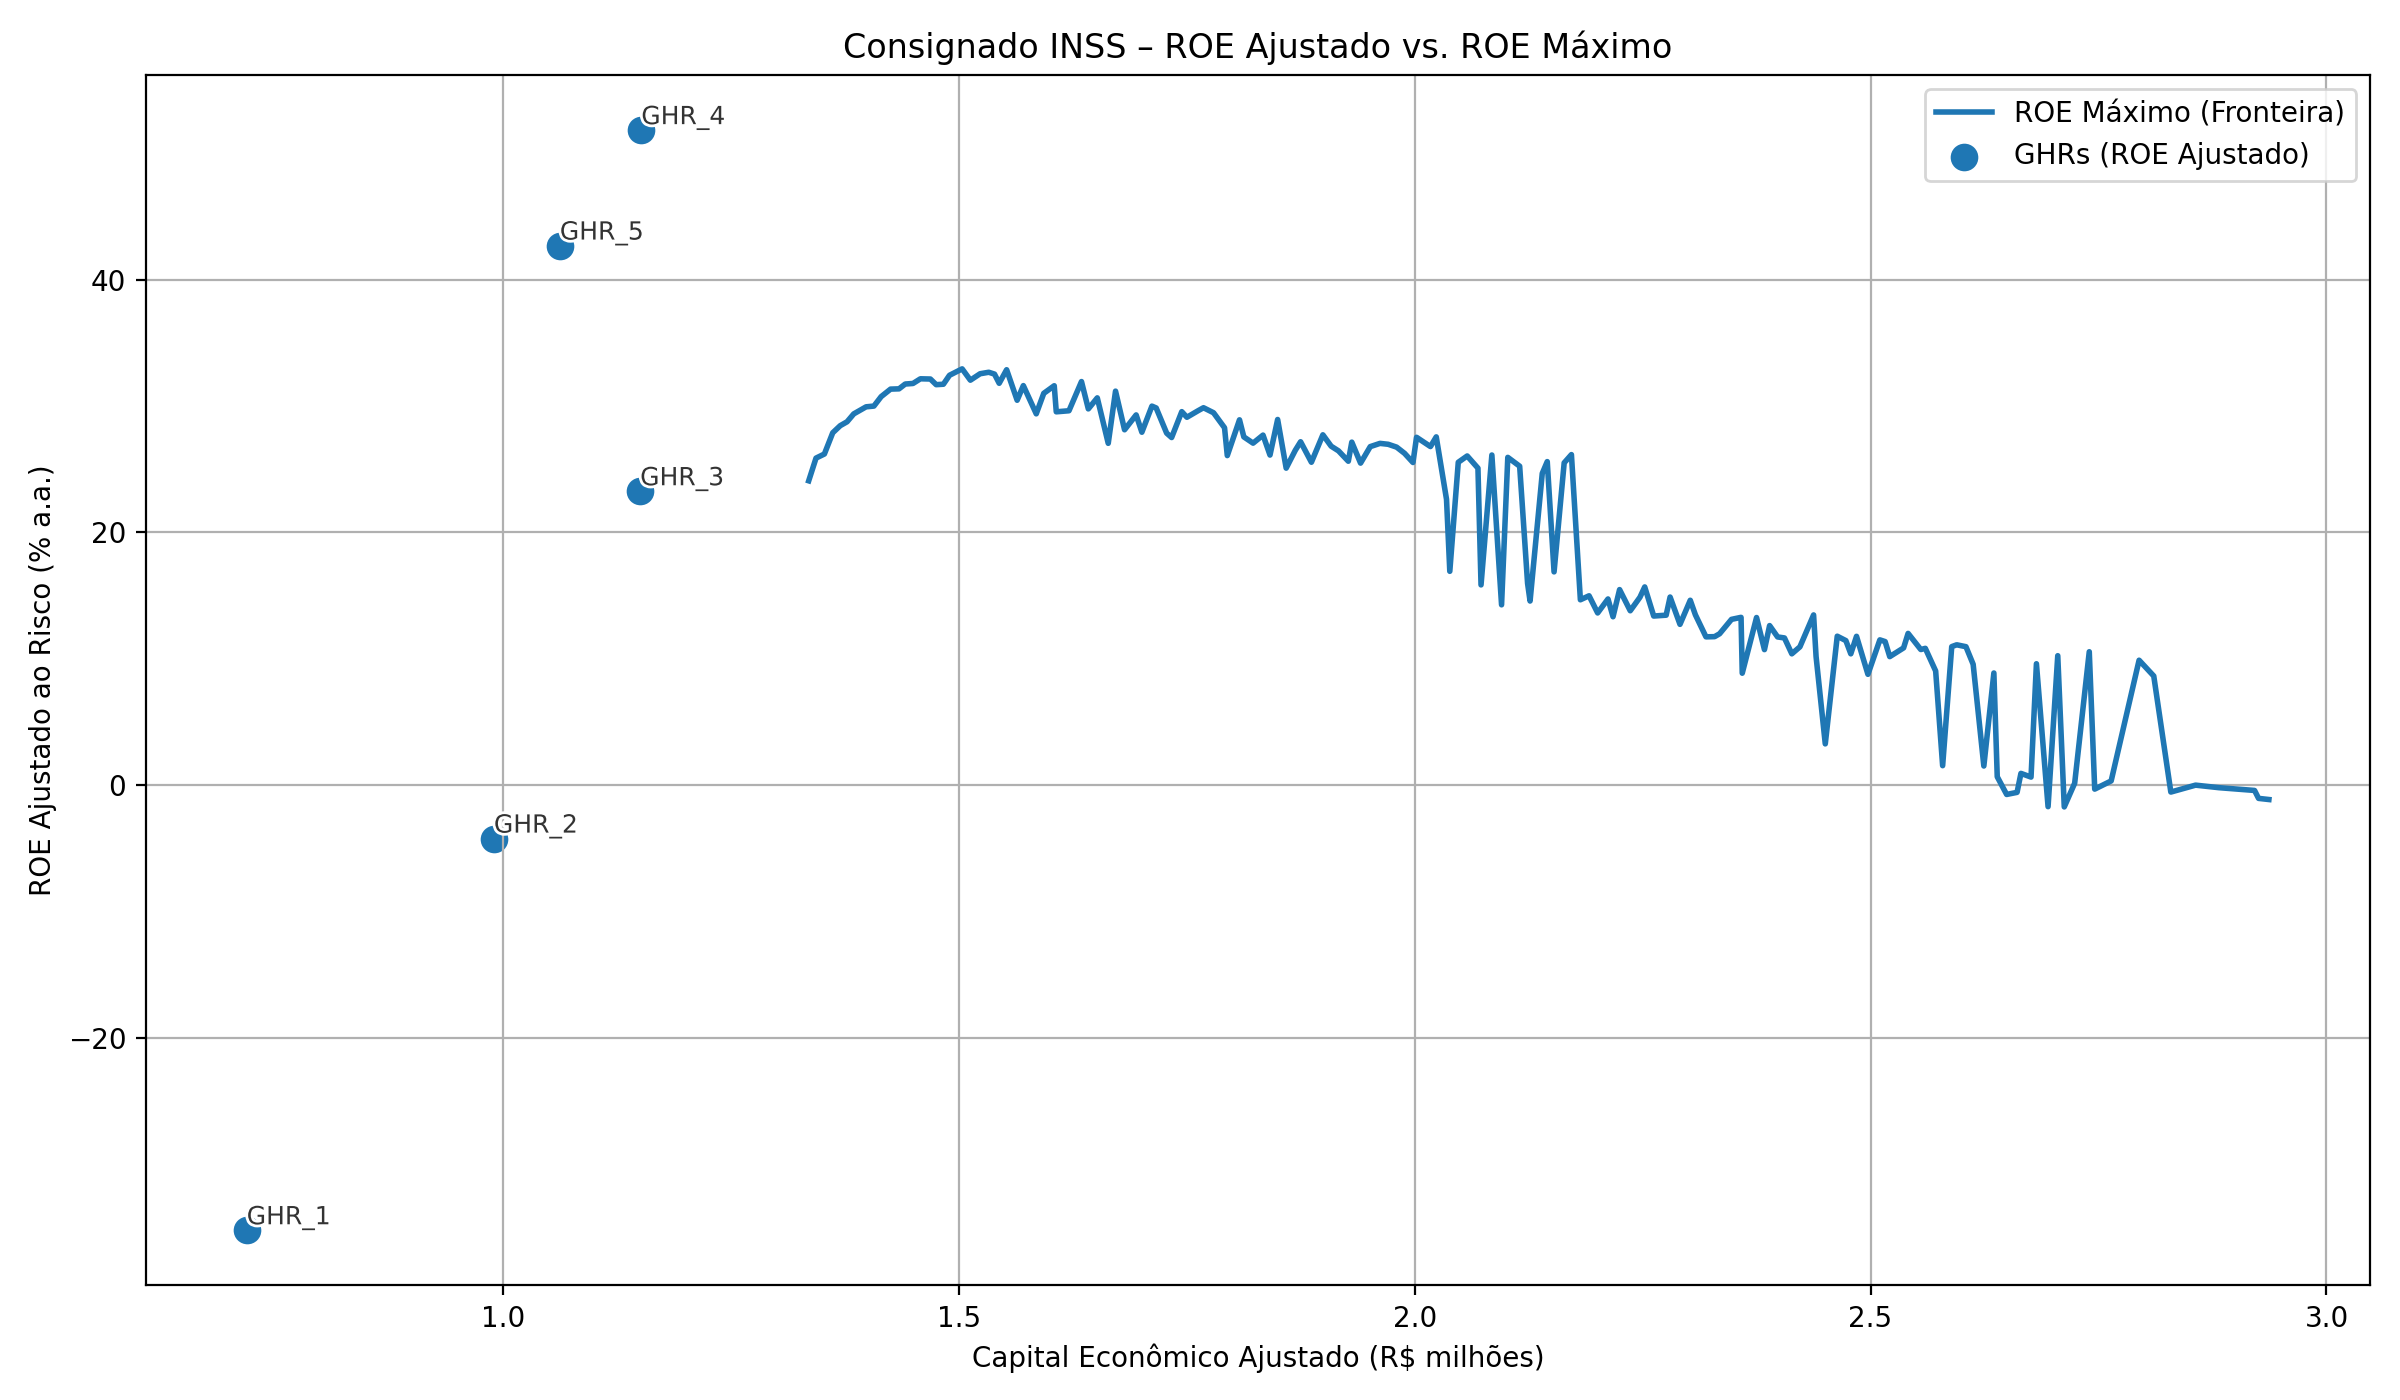
\includegraphics[width=.85\linewidth]{roe_maximo.png}
\caption{ROE Ajustado vs. ROE Máximo – Visão Total.}
\end{figure}

\subsection*{Visão Sem Safra}
\begin{figure}[H]\centering
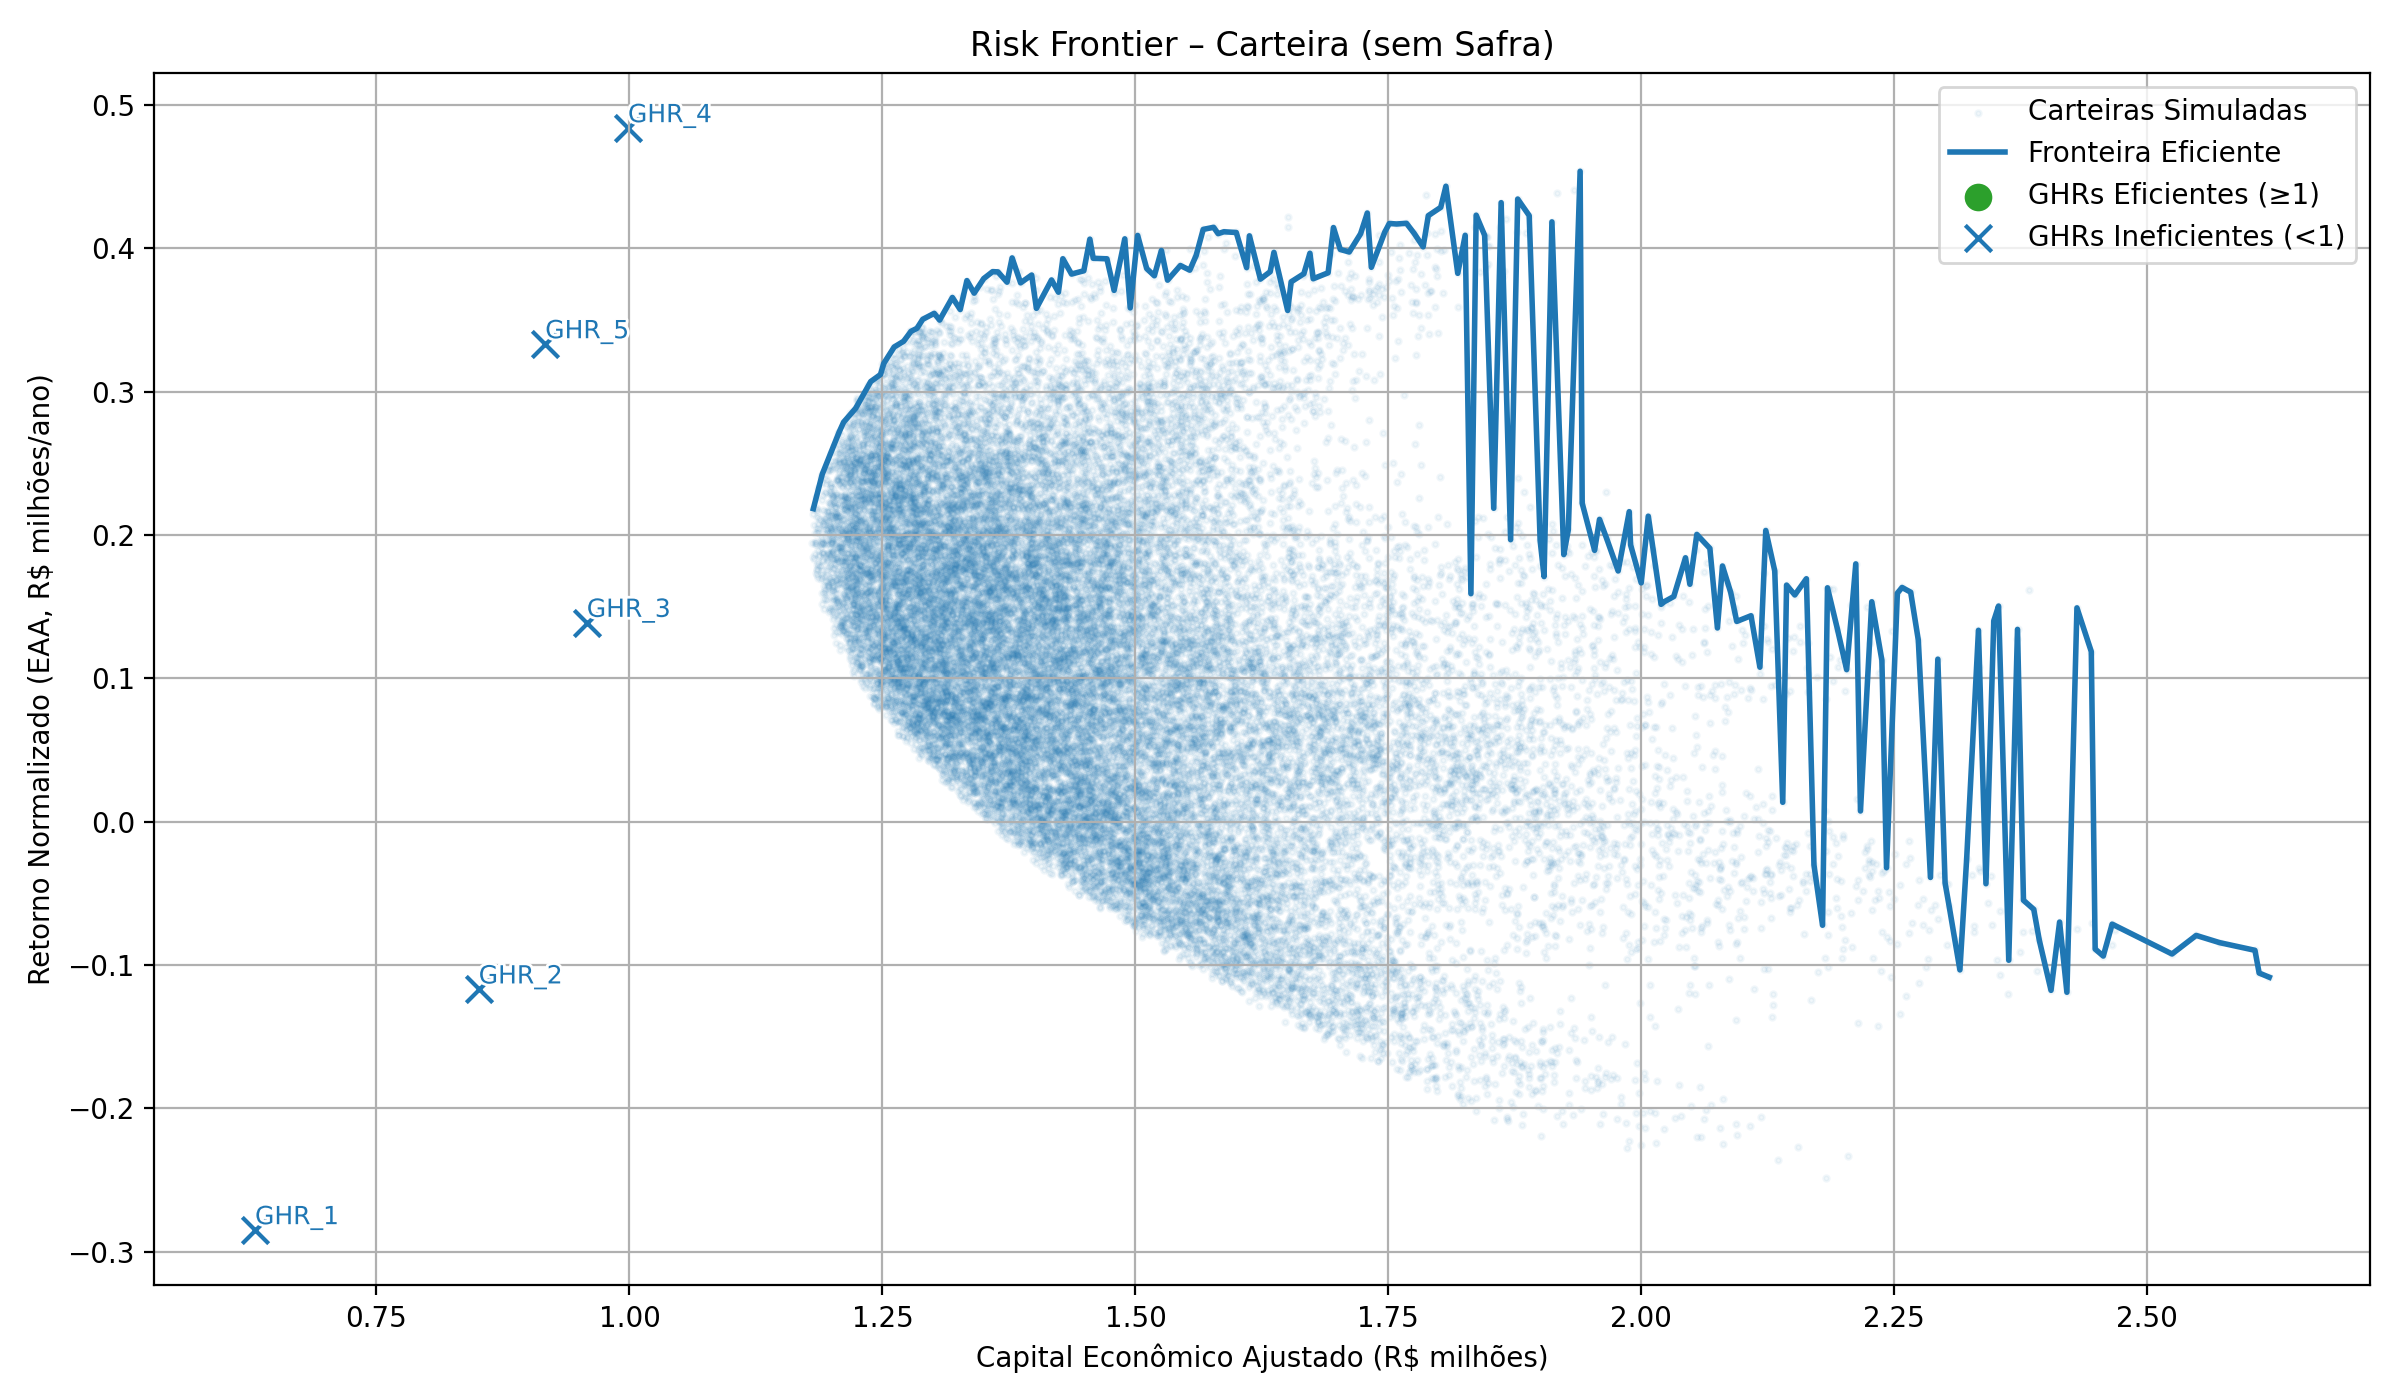
\includegraphics[width=.85\linewidth]{fronteira_sem_safra.png}
\caption{Fronteira eficiente – Carteira \emph{sem} Safra.}
\end{figure}

\begin{figure}[H]\centering
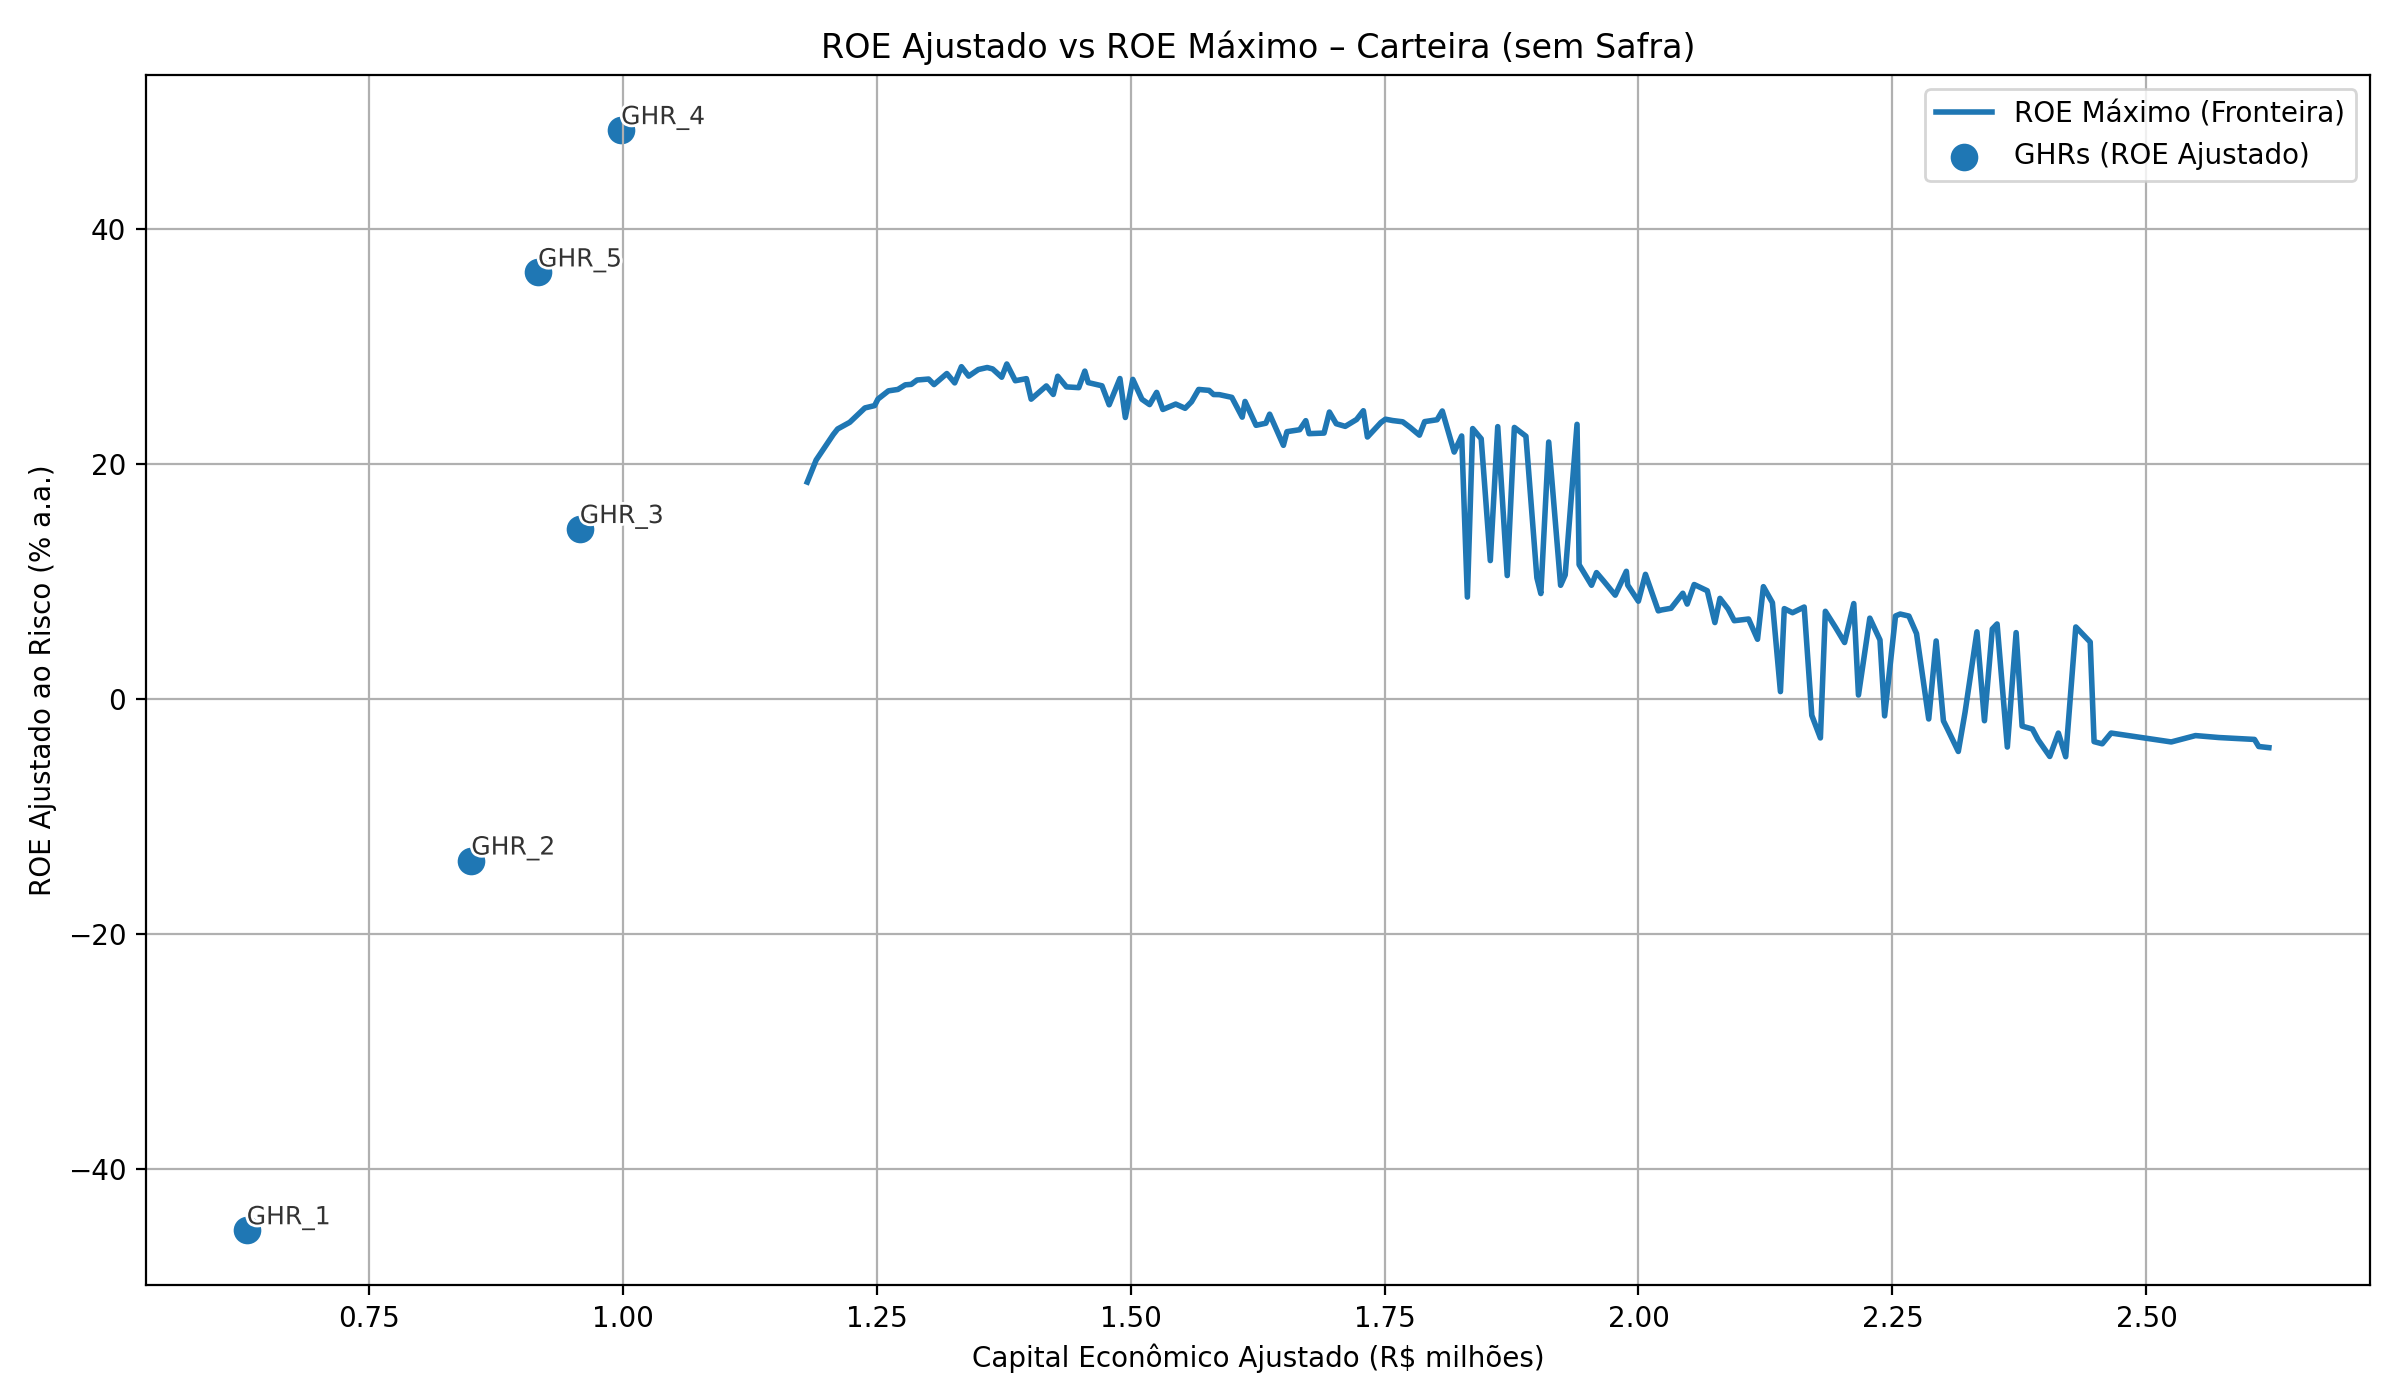
\includegraphics[width=.85\linewidth]{roe_maximo_sem_safra.png}
\caption{ROE Ajustado vs. ROE Máximo – Carteira \emph{sem} Safra.}
\end{figure}

\subsection*{Visão Só Safra}
\begin{figure}[H]\centering
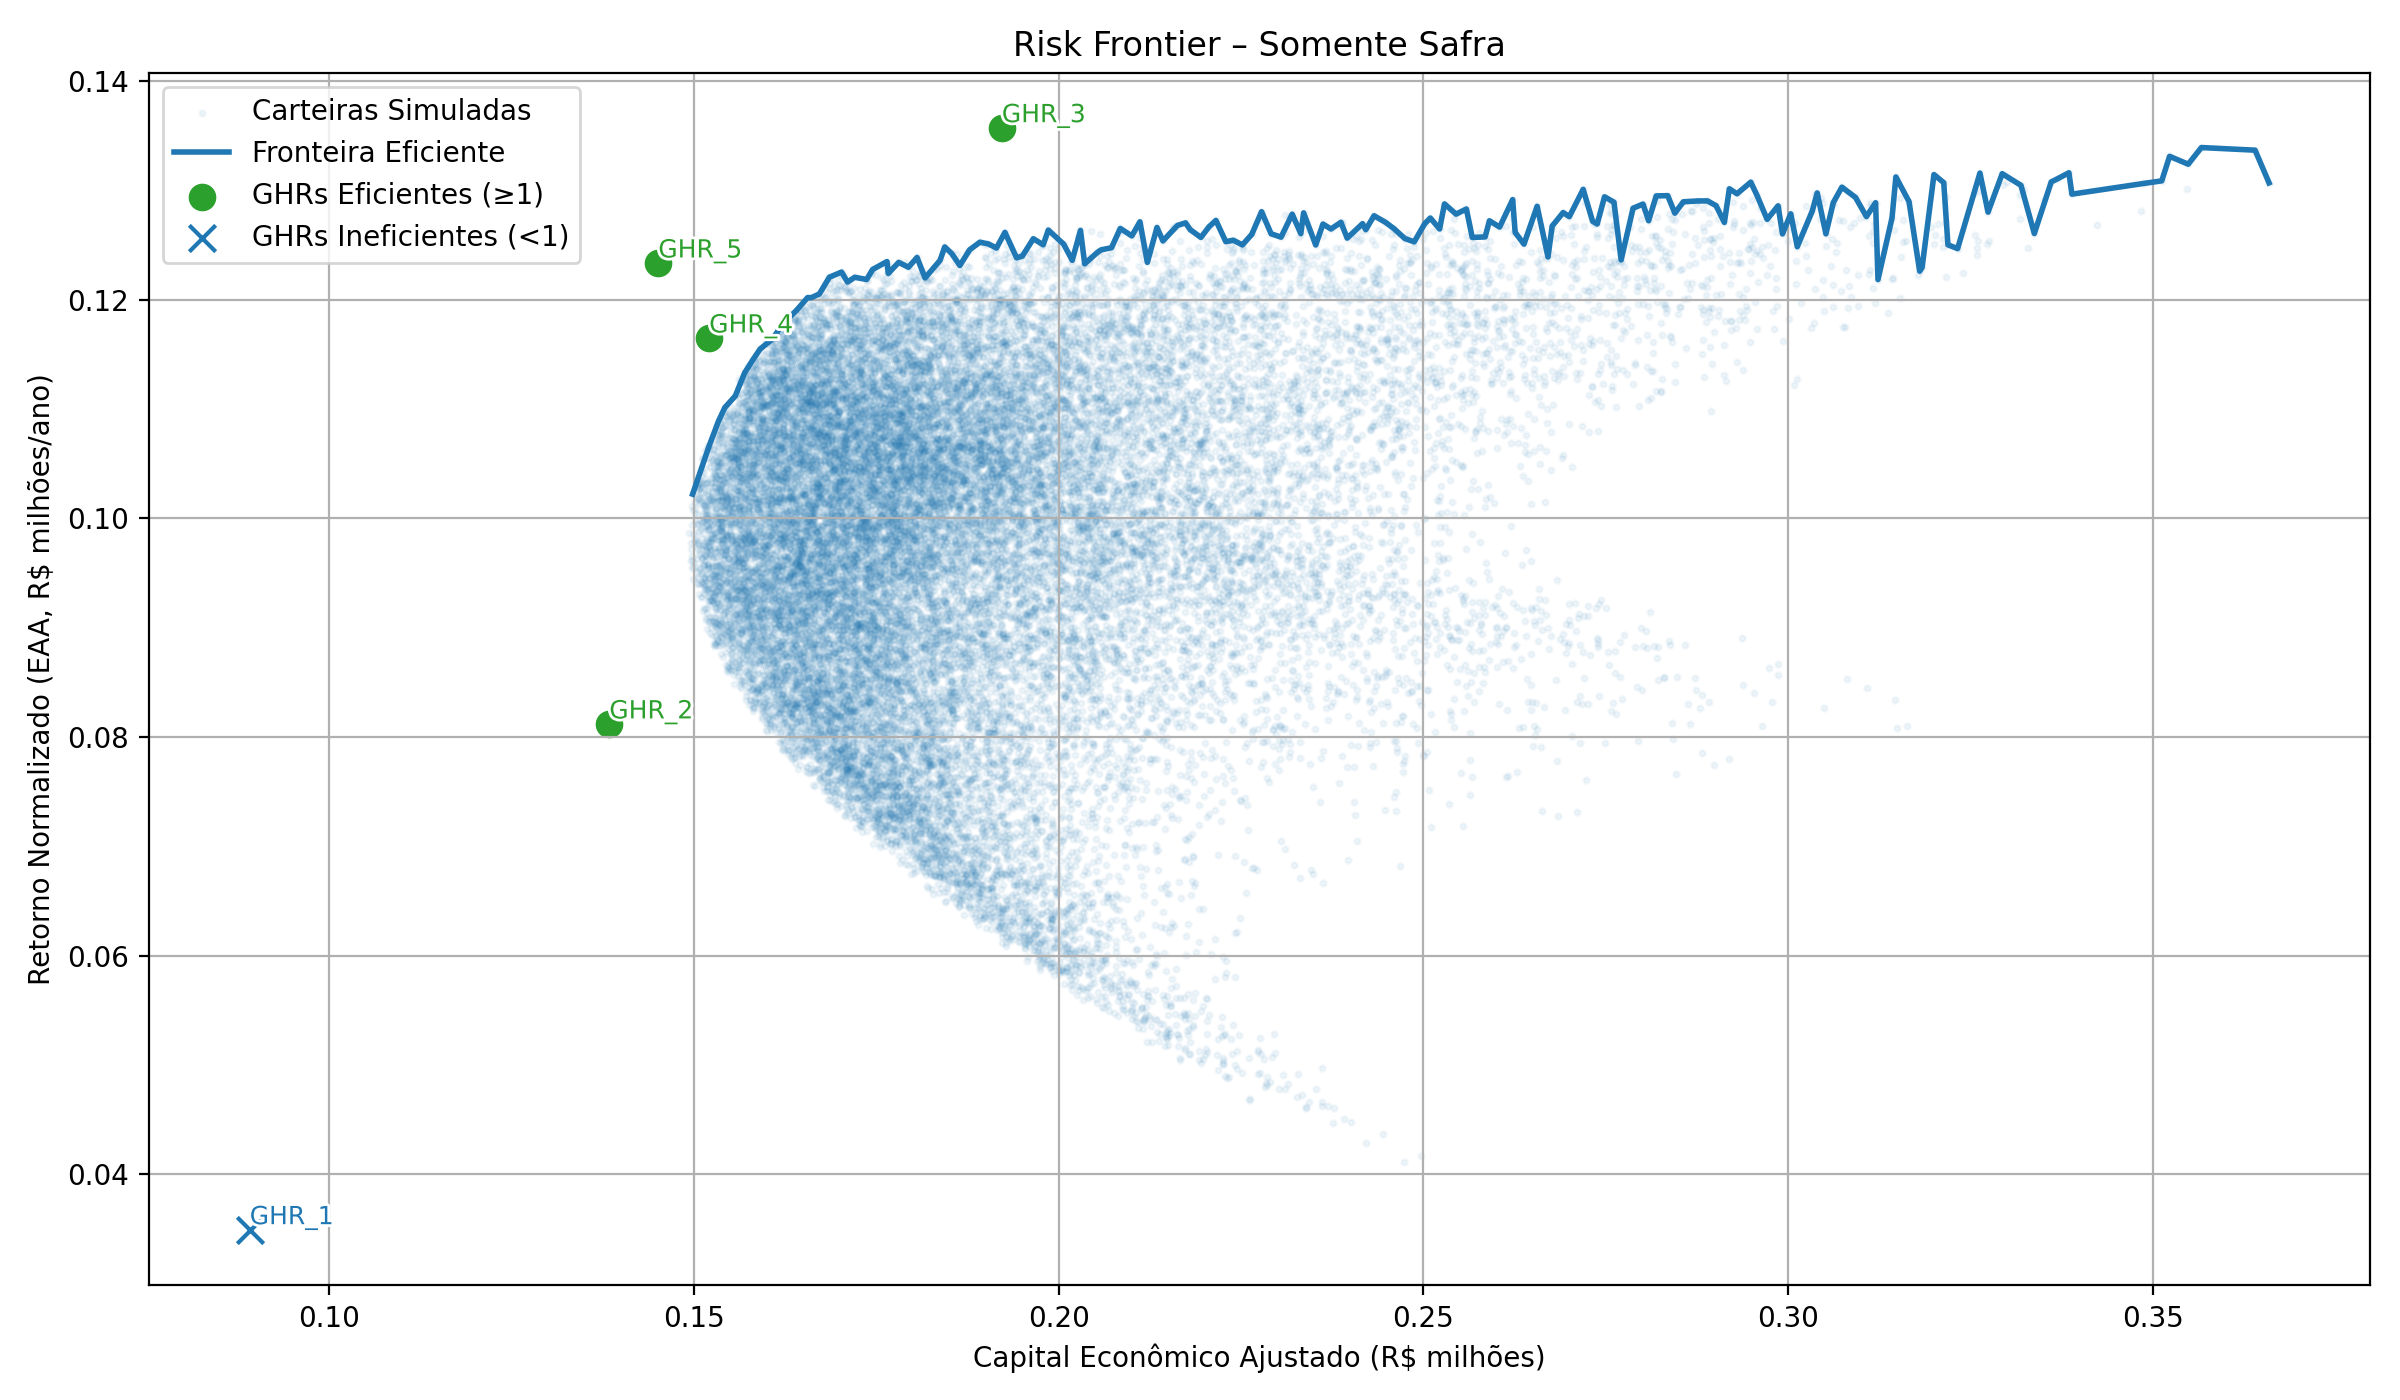
\includegraphics[width=.85\linewidth]{fronteira_safra.png}
\caption{Fronteira eficiente – \emph{Somente} Safra.}
\end{figure}

\begin{figure}[H]\centering
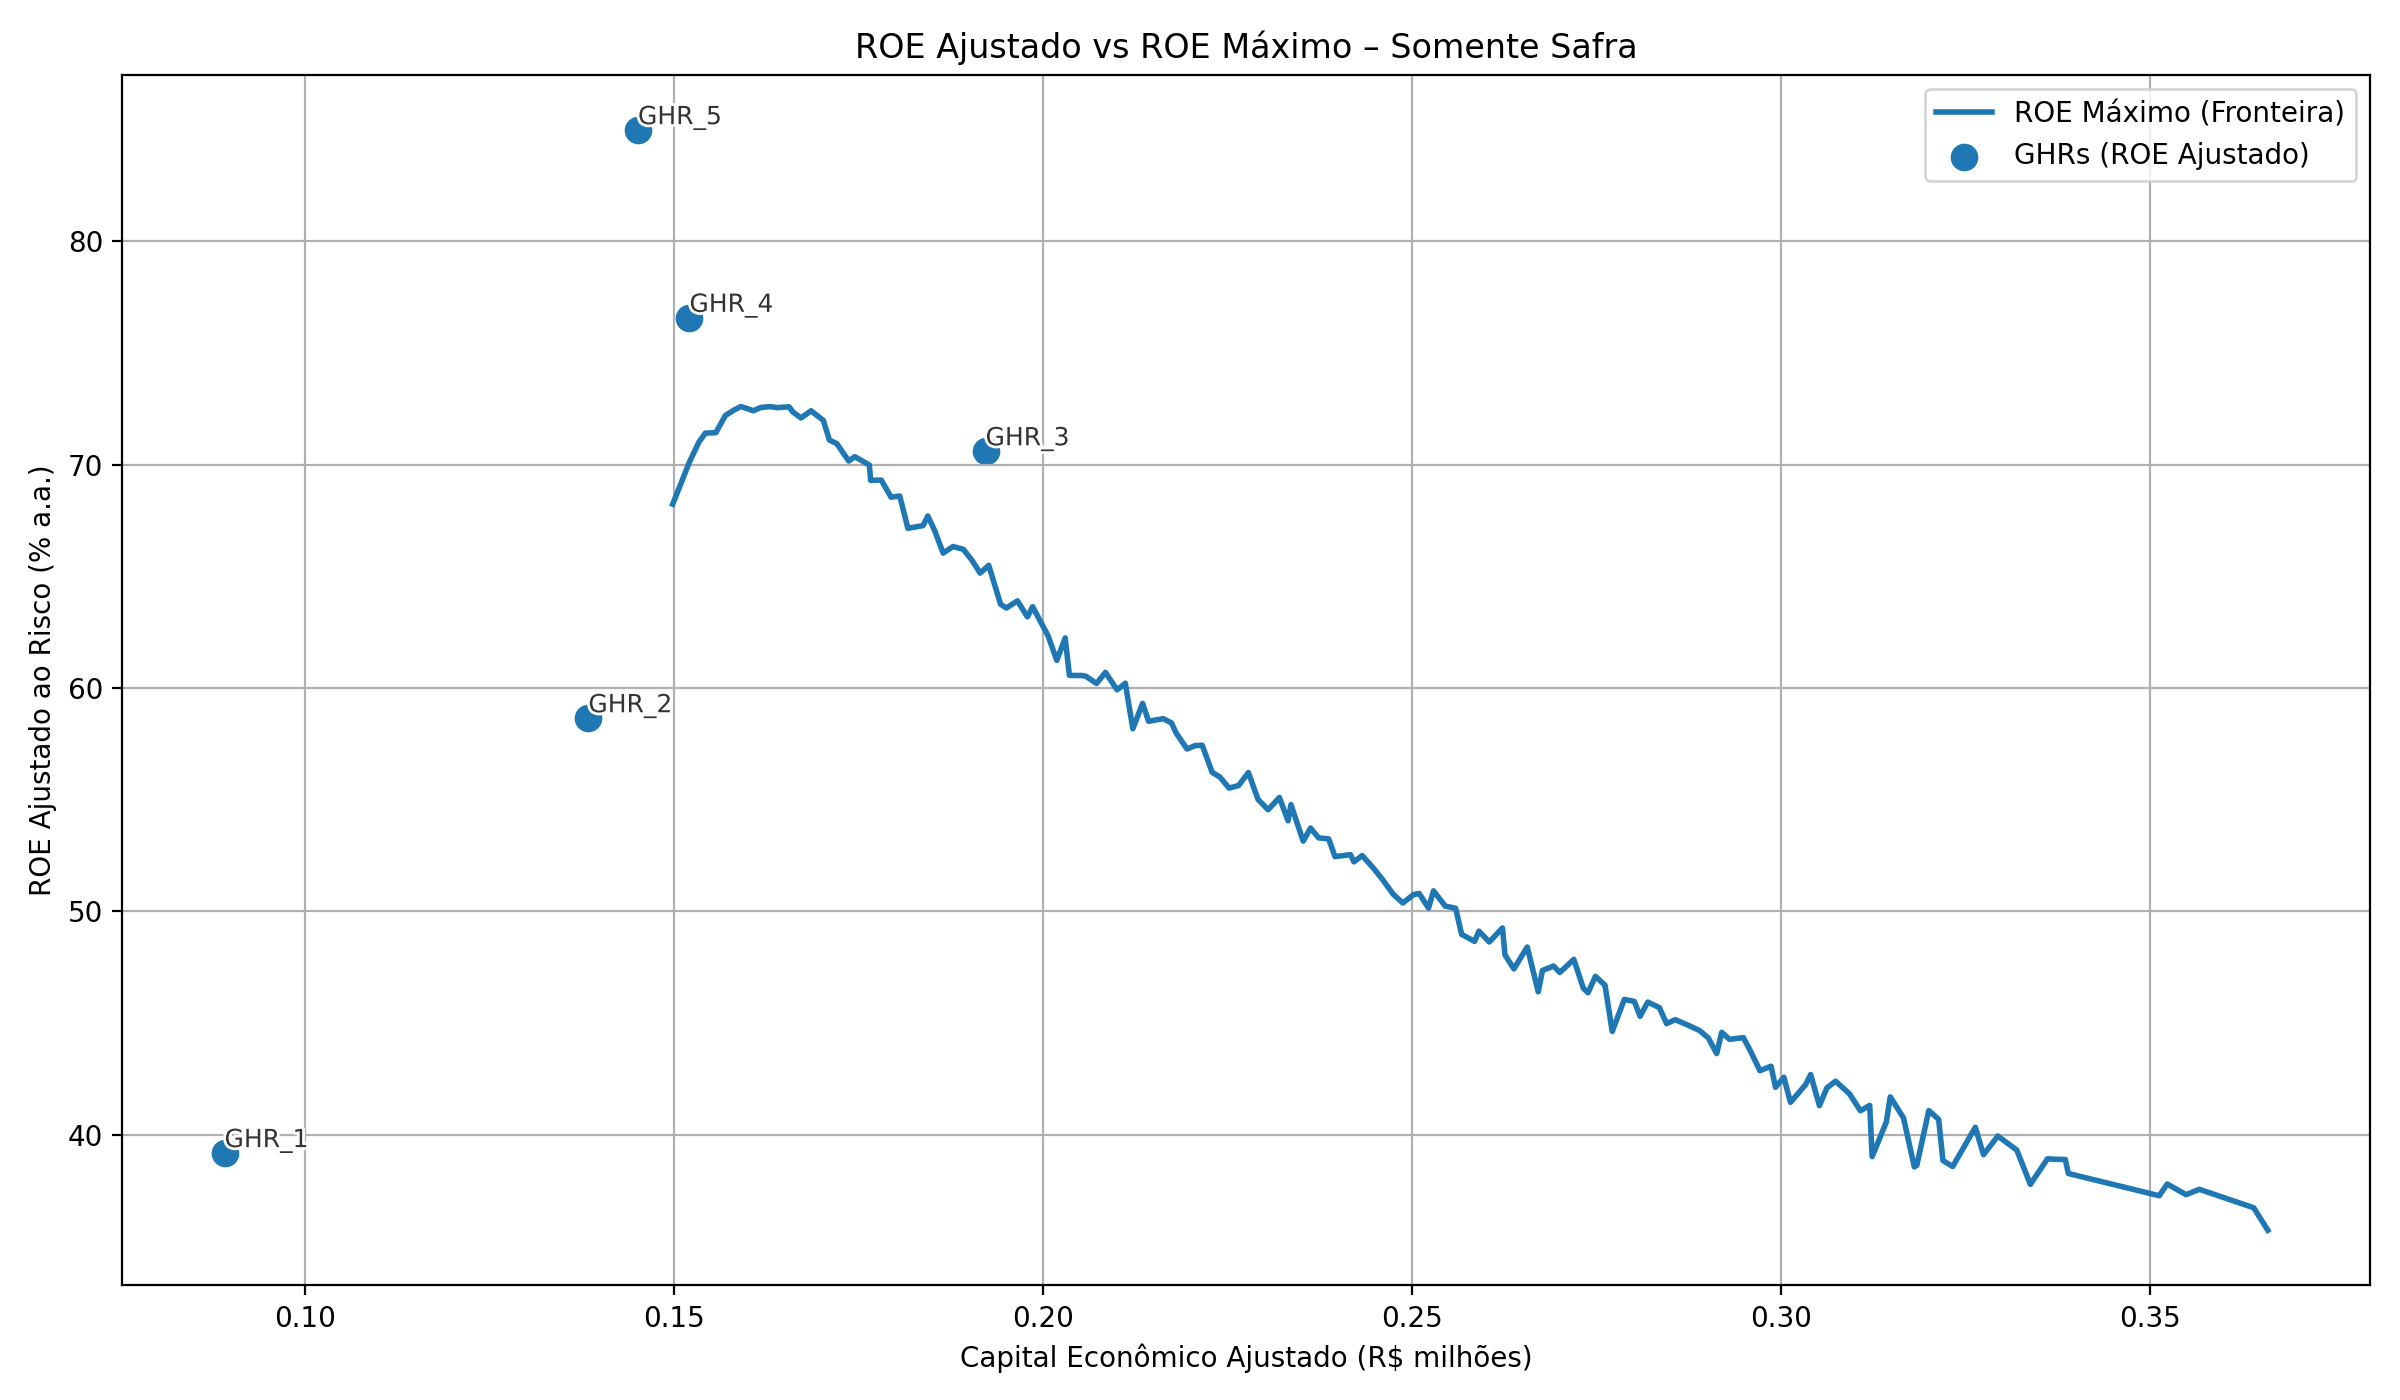
\includegraphics[width=.85\linewidth]{roe_maximo_safra.png}
\caption{ROE Ajustado vs. ROE Máximo – \emph{Somente} Safra.}
\end{figure}

% ============================================================
\section*{Referências (essenciais)}
\begin{itemize}[noitemsep]
  \item Basel Committee on Banking Supervision (BCBS). \emph{International Convergence of Capital Measurement and Capital Standards}.
  \item Vasicek, O. (2002). \emph{Loan Portfolio Value}. \textit{RISK}.
  \item Modelagem de roll-rates (cadeias de Markov) em gerenciamento de crédito.
\end{itemize}

\clearpage
\appendix
\section{Script Python completo}
\noindent Abaixo, o script usado (mesma versão que salva os PNGs mencionados). Ajuste apenas \texttt{INPUT\_XLSX} e \texttt{OUTPUT\_DIR} conforme seu ambiente.
\begin{lstlisting}[language=Python, caption={risk_frontier.py (versão completa com normalização por prazo e visões)}]
# ================================================================
# Risk Frontier – Consignado INSS (apenas contratos ATIVOS)
# Versão "Delinquency-aware" + Normalização por Prazo (anual/12m/EAA)
# Entradas obrigatórias: 'contratos', 'ghr_param', 'params'
# Opcionais: 'roll_rates','prov_reg','lgd_bucket','opex_cobranca','rho_mult_bucket'
# Saídas: Excel consolidado + gráficos PNG (Total, Sem Safra, Só Safra)
# Requisitos: numpy, pandas, matplotlib, scipy, xlsxwriter
# ================================================================

import numpy as np
import pandas as pd
import matplotlib.pyplot as plt
import matplotlib.patheffects as pe
from scipy.stats import norm
from scipy.interpolate import interp1d
from pathlib import Path

# ---------- Config ----------
INPUT_XLSX = r"<>\INPUT.xlsx"
OUTPUT_DIR = Path(r"<>")
OUTPUT_DIR.mkdir(parents=True, exist_ok=True)
OUT_XLSX = OUTPUT_DIR / "risk_frontier_relatorio.xlsx"

SEED = 20250812
np.random.seed(SEED)
CONF_LEVEL = 0.999
Z_ALPHA = norm.ppf(CONF_LEVEL)

RHO_PADRAO = 0.12
PD_FLOOR, PD_CAP = 0.001, 0.30
LGD_FLOOR, LGD_CAP = 0.05, 0.50
ALPHA_OVERS, ALPHA_DELAY = 0.7, 0.3
FUNDING_AA_DEFAULT = 0.10
H_FWD_MESES_DEFAULT = 12

ESTADOS_ATIVOS = {"Em dia", "Em atraso", "Na Safra"}
BUCKETS = ["current","30","60","90","wo"]  # tudo minúsculo!

# ---- Normalização por prazo ----
MODO_PRAZO = "eaa"     # "anual" | "12m" | "eaa"
K_EAA = 0.12           # taxa a.a. p/ EAA
M_PISO_ANOS = 0.25     # piso de prazo médio

# ---------- Funções ----------
def pd_dinamico(pd_base, overs, is_delayed, alpha_overs=ALPHA_OVERS, alpha_delay=ALPHA_DELAY):
    fator = 1 + alpha_overs * overs + alpha_delay * is_delayed
    return float(np.clip(pd_base * fator, PD_FLOOR, PD_CAP))

def vasicek_ul(pd, lgd, ead, rho, z=Z_ALPHA):
    inv_pd  = norm.ppf(pd)
    cond_pd = norm.cdf((inv_pd + np.sqrt(rho) * z) / np.sqrt(1 - rho))
    return float(lgd * ead * cond_pd)

def basel_maturity_adjustment(pd, k_1y, m_years):
    pd_clip = np.clip(pd, PD_FLOOR, 0.5)
    b = (0.11852 - 0.05478 * np.log(pd_clip)) / (1 - 0.11852 - 0.05478 * np.log(pd_clip))
    fator_m = (1 + (m_years - 2.5) * b) / (1 - 1.5 * b)
    return float(max(k_1y * max(fator_m, 0.1), 0.0))

def pmt_price(valor, i_mensal, n_meses):
    if i_mensal == 0:
        return valor / max(n_meses, 1)
    return valor * (i_mensal * (1 + i_mensal)**n_meses) / ((1 + i_mensal)**n_meses - 1)

def saldo_price(valor, i_mensal, n_total, n_pag):
    if i_mensal == 0:
        return float(max(valor - (valor / max(n_total, 1)) * n_pag, 0.0))
    pmt = pmt_price(valor, i_mensal, n_total)
    saldo = valor * (1 + i_mensal)**n_pag - pmt * ((1 + i_mensal)**n_pag - 1) / i_mensal
    return float(max(saldo, 0.0))

def construir_fronteira(EAD, LGD, EL_1y, RetLiq_1y, rho_mat, n_points=30000, seed=SEED):
    rng = np.random.default_rng(seed)
    n = len(EAD)
    if n == 0:
        return np.array([]), np.array([]), np.array([]), np.array([])
    if n == 1:
        ecs = np.array([np.sqrt((LGD[0]*EAD[0])**2 * rho_mat[0,0])])
        rets = np.array([RetLiq_1y[0] - EL_1y[0]])
        return ecs, rets, ecs, rets
    weights = rng.dirichlet(np.ones(n), n_points)
    ecs, rets = [], []
    for w in weights:
        ead_w = w * EAD
        losses_scale = LGD * ead_w
        cov = np.outer(losses_scale, losses_scale) * rho_mat
        ec_total = np.sqrt(np.sum(cov))
        el_total = np.sum(w * EL_1y)
        ret_total = np.sum(w * (RetLiq_1y + EL_1y))
        rets.append(ret_total - el_total)
        ecs.append(ec_total)
    ecs = np.array(ecs); rets = np.array(rets)
    grid = np.linspace(ecs.min(), ecs.max(), 180)
    fr_ec, fr_ret = [], []
    tol = (ecs.max() - ecs.min()) / 400
    for g in grid:
        mask = (ecs >= g - tol) & (ecs <= g + tol)
        if np.any(mask):
            i = np.argmax(rets[mask])
            fr_ec.append(ecs[mask][i]); fr_ret.append(rets[mask][i])
    return np.array(fr_ec), np.array(fr_ret), ecs, rets

# ---- Defaults de delinquency ----
ROLL_DEFAULT = pd.DataFrame({
    "current":[0.92, 0.06, 0.01, 0.00, 0.01],
    "30"     :[0.35, 0.45, 0.15, 0.02, 0.03],
    "60"     :[0.10, 0.25, 0.45, 0.15, 0.05],
    "90"     :[0.02, 0.05, 0.28, 0.45, 0.20],
    "wo"     :[0.00, 0.00, 0.00, 0.00, 1.00],
}, index=BUCKETS)
PROV_REG_DEFAULT  = pd.DataFrame({"bucket":BUCKETS,"pct":[0.02,0.10,0.30,0.50,1.00]})
LGD_BUCKET_DEFAULT= pd.DataFrame({"bucket":BUCKETS,"lgd":[0.25,0.30,0.35,0.40,0.45]})
OPEX_DEFAULT      = pd.DataFrame({"bucket":BUCKETS,"opex":[0.0,15.0,22.0,35.0,80.0]})
RHO_MULT_DEFAULT  = pd.DataFrame({"bucket":BUCKETS,"rho_mult":[1.00,1.05,1.10,1.15,1.20]})

# ---- Helpers ----
def _lower_cols(df): df.columns = df.columns.str.strip().str.lower(); return df
def _lower_index(df): df.index = df.index.map(lambda x: str(x).strip().lower()); return df

def ler_tabela_ou_default(xls, sheet, default_df):
    try:
        df = pd.read_excel(xls, sheet)
        return _lower_cols(df)
    except Exception:
        return default_df.copy()

def load_roll_rates_strict(xls, sheet_name, default_df, buckets):
    try:
        df = pd.read_excel(xls, sheet_name)
        df = _lower_cols(df)
    except Exception:
        df = default_df.copy()
    df = df.loc[:, ~df.columns.astype(str).str.contains("^unnamed", case=False, regex=True)]
    cand_idx = None
    for c in df.columns:
        if str(c).strip().lower() in ["bucket","bkt","estado","faixa","bucket_atraso"]:
            cand_idx = c; break
    if cand_idx is not None:
        df = df.set_index(cand_idx)
    df = _lower_index(df)
    if set(buckets).issubset(set(df.columns)):
        df = df[buckets]
    elif set(buckets).issubset(set(df.index)):
        df = df.loc[buckets].T
    df = df.reindex(index=buckets, columns=buckets)
    df = df.apply(pd.to_numeric, errors="coerce").fillna(0.0)
    for i in df.index:
        if i == "wo":
            df.loc[i] = 0.0; df.loc[i,"wo"] = 1.0
        else:
            s = df.loc[i].sum()
            df.loc[i] = (df.loc[i] / s) if s > 0 else 0.0
            if s == 0: df.loc[i, i] = 1.0
    return df

def pd_condicional_from_roll(start_bucket, horizon_m, roll_df):
    idx = {b:i for i,b in enumerate(roll_df.index)}
    state = np.zeros(len(roll_df)); state[idx[start_bucket]] = 1.0
    p_default = 0.0
    P = roll_df.values
    wo_col = roll_df.columns.get_loc("wo")
    for _ in range(horizon_m):
        p_default += state @ P[:, wo_col]
        state = state @ P
        state[idx["wo"]] = 0.0
    return float(np.clip(p_default, 0.0, 1.0))

def expected_carry_cost(EAD, bucket, funding_aa, spread_aa, months, opex_map, suspende_accrual=True):
    funding_am = (1 + funding_aa)**(1/12) - 1
    spread_am  = (1 + spread_aa )**(1/12) - 1
    lost_rev   = spread_am * EAD if suspende_accrual else 0.0
    carry_m    = funding_am * EAD + lost_rev + opex_map.get(bucket, 0.0)
    return carry_m * months

# ---------- 1) Ler entrada ----------
xls = pd.ExcelFile(INPUT_XLSX)
contratos = pd.read_excel(xls, "contratos")
ghr_param = pd.read_excel(xls, "ghr_param")
try:
    params = pd.read_excel(xls, "params")
except Exception:
    params = None

# opcionais
roll_df     = load_roll_rates_strict(xls, "roll_rates", ROLL_DEFAULT, BUCKETS)
prov_reg_df = ler_tabela_ou_default(xls, "prov_reg", PROV_REG_DEFAULT)
lgd_bkt_df  = ler_tabela_ou_default(xls, "lgd_bucket", LGD_BUCKET_DEFAULT)
opex_df     = ler_tabela_ou_default(xls, "opex_cobranca", OPEX_DEFAULT)
rho_mult_df = ler_tabela_ou_default(xls, "rho_mult_bucket", RHO_MULT_DEFAULT)

prov_reg_df = _lower_cols(prov_reg_df); lgd_bkt_df = _lower_cols(lgd_bkt_df)
opex_df     = _lower_cols(opex_df);     rho_mult_df= _lower_cols(rho_mult_df)
prov_map = dict(zip(prov_reg_df["bucket"], prov_reg_df["pct"]))
lgd_map  = dict(zip(lgd_bkt_df["bucket"],  lgd_bkt_df["lgd"]))
opex_map = dict(zip(opex_df["bucket"],     opex_df["opex"]))
rho_mult = dict(zip(rho_mult_df["bucket"], rho_mult_df["rho_mult"]))

funding_aa  = FUNDING_AA_DEFAULT
H_FWD_MESES = H_FWD_MESES_DEFAULT
if params is not None and {"Parametro","Valor"}.issubset(params.columns):
    mparams = params.set_index("Parametro")["Valor"].to_dict()
    try: funding_aa  = float(mparams.get("Funding_aa", FUNDING_AA_DEFAULT))
    except: pass
    try: H_FWD_MESES = int(mparams.get("H_fwd_meses", H_FWD_MESES_DEFAULT))
    except: pass
    if "Modo_prazo" in mparams:
        MODO_PRAZO = str(mparams["Modo_prazo"]).strip().lower()
    if "K_EAA" in mparams:
        try: K_EAA = float(mparams["K_EAA"])
        except: pass

# ---------- PATCH Spread_aa ----------
def _norm_cols_keepcase(df):
    df.columns = df.columns.str.strip()
    return df
contratos = _norm_cols_keepcase(contratos)
ghr_param = _norm_cols_keepcase(ghr_param)
alt_names = {"spread":"Spread_aa","Spread aa":"Spread_aa","spread_aa":"Spread_aa","SPREAD_AA":"Spread_aa"}
contratos.rename(columns={k:v for k,v in alt_names.items() if k in contratos.columns}, inplace=True)
ghr_param.rename(columns={k:v for k,v in alt_names.items() if k in ghr_param.columns}, inplace=True)

if "GHR" not in contratos.columns or "GHR" not in ghr_param.columns:
    raise ValueError("A coluna 'GHR' deve existir em 'contratos' e 'ghr_param'.")
contratos["GHR"] = contratos["GHR"].astype(str).str.strip()
ghr_param["GHR"] = ghr_param["GHR"].astype(str).str.strip()

need_cols = {"PD_Base","LGD_Base","Spread_aa"}
if not need_cols.issubset(contratos.columns):
    cols_to_bring = ["GHR"] + [c for c in ["PD_Base","LGD_Base","Spread_aa"] if c in ghr_param.columns]
    contratos = contratos.merge(ghr_param[cols_to_bring], on="GHR", how="left", validate="many_to_one")

if "Spread_aa" not in contratos.columns or contratos["Spread_aa"].isna().all():
    if "Spread_aa" in ghr_param.columns and not ghr_param["Spread_aa"].isna().all():
        contratos["Spread_aa"] = contratos["GHR"].map(dict(zip(ghr_param["GHR"], ghr_param["Spread_aa"])))
    if "Spread_aa" not in contratos.columns:
        contratos["Spread_aa"] = np.nan
    if contratos["Spread_aa"].isna().any():
        ghrs = sorted(contratos["GHR"].unique())
        defaults = [0.14,0.16,0.18,0.20,0.22]
        while len(defaults) < len(ghrs): defaults.append(defaults[-1])
        contratos["Spread_aa"] = contratos["Spread_aa"].fillna(contratos["GHR"].map({g:s for g,s in zip(ghrs, defaults)}))
    contratos["Spread_aa"] = contratos["Spread_aa"].fillna(0.18)
if contratos["Spread_aa"].isna().any():
    raise ValueError("Não foi possível determinar 'Spread_aa' para alguns contratos.")

# ---------- 2) Pré-processamento ----------
contratos = contratos[contratos["Estado"].isin(ESTADOS_ATIVOS)].copy()
req_cols = {"ContratoID","GHR","Estado","Valor_Liberado","Prazo_Meses","Meses_Pagos"}
missing = req_cols - set(contratos.columns)
if missing:
    raise ValueError(f"Faltam colunas em 'contratos': {missing}")

contratos["Meses_Pagos"] = contratos.apply(
    lambda r: 0 if r["Estado"]=="Na Safra" else min(max(int(r["Meses_Pagos"]), 0), int(r["Prazo_Meses"])-1), axis=1
)
contratos["Meses_Restantes"] = contratos["Prazo_Meses"] - contratos["Meses_Pagos"]
contratos = contratos[contratos["Meses_Restantes"] > 0].copy()

contratos["Juros_aa"] = funding_aa + contratos["Spread_aa"]
contratos["Juros_am"] = (1 + contratos["Juros_aa"])**(1/12) - 1

if "Saldo_Atual" in contratos.columns:
    contratos["Saldo"] = contratos["Saldo_Atual"].astype(float)
else:
    contratos["Saldo"] = [
        saldo_price(v, i, n, p)
        for v, i, n, p in zip(contratos["Valor_Liberado"], contratos["Juros_am"], contratos["Prazo_Meses"], contratos["Meses_Pagos"])
    ]

def infer_bucket(row):
    if "Bucket_Atraso" in contratos.columns and pd.notnull(row.get("Bucket_Atraso")):
        b = str(row["Bucket_Atraso"]).strip().lower()
        return "current" if b in ["0","cur","current"] else b
    if "DPD" in contratos.columns and pd.notnull(row.get("DPD")):
        d = int(row["DPD"])
        if d <= 0: return "current"
        if d <= 30: return "30"
        if d <= 60: return "60"
        if d <= 90: return "90"
        return "wo"
    if row["Estado"] in ["Em dia","Na Safra"]: return "current"
    return "30"
contratos["bucket"] = contratos.apply(infer_bucket, axis=1)

if "Overs_Flag" not in contratos.columns or "IsDelayed_Flag" not in contratos.columns:
    rng = np.random.default_rng(SEED)
    overs_prob = np.where(
        contratos["Estado"].eq("Em atraso"), rng.uniform(0.20,0.50, len(contratos)),
        np.where(contratos["Estado"].eq("Na Safra"), rng.uniform(0.05,0.15, len(contratos)),
                 rng.uniform(0.00,0.05, len(contratos)))
    )
    isdel_prob = np.where(
        contratos["Estado"].eq("Em atraso"), rng.uniform(0.10,0.30, len(contratos)),
        np.where(contratos["Estado"].eq("Na Safra"), rng.uniform(0.05,0.20, len(contratos)),
                 rng.uniform(0.01,0.08, len(contratos)))
    )
    contratos["Overs_Flag"]     = rng.random(len(contratos)) < overs_prob
    contratos["IsDelayed_Flag"] = rng.random(len(contratos)) < isdel_prob

# ---------- 3) Agregado por GHR ----------
agg = []
for ghr, sub in contratos.groupby("GHR"):
    ead = sub["Saldo"].sum()
    vol = len(sub)
    pd_base  = float(sub["PD_Base"].iloc[0])
    lgd_base = float(sub["LGD_Base"].iloc[0])
    spread   = float(sub["Spread_aa"].iloc[0])
    overs    = float(sub["Overs_Flag"].mean())
    isdel    = float(sub["IsDelayed_Flag"].mean())
    m_rem_anos = float(np.average(sub["Meses_Restantes"], weights=sub["Saldo"]) / 12.0) if ead > 0 else 0.0
    pd_adj = pd_dinamico(pd_base, overs, isdel)

    el_mes_total = 0.0
    lgd_eff_weighted = 0.0
    rho_mult_w = 0.0
    for _, r in sub.iterrows():
        EADi = float(r["Saldo"]); bkt  = str(r["bucket"]).strip().lower()
        prov_inc = float(prov_map.get(bkt, 0.0)) * EADi
        H_i  = int(min(H_FWD_MESES, r["Meses_Restantes"]))
        pd_fwd = pd_condicional_from_roll(bkt, H_i, roll_df)
        lgd_b = float(np.clip(lgd_map.get(bkt, lgd_base), LGD_FLOOR, LGD_CAP))
        ecl_fwd = pd_fwd * lgd_b * EADi
        susp = (bkt != "current")
        carry = expected_carry_cost(EADi, bkt, funding_aa, spread, months=H_i, opex_map=opex_map, suspende_accrual=susp)
        el_mes_total += (prov_inc + ecl_fwd + carry)
        lgd_eff_weighted += lgd_b * EADi
        rho_mult_w += rho_mult.get(bkt, 1.0) * EADi

    lgd_eff = (lgd_eff_weighted / ead) if ead > 0 else lgd_base
    rho_eff = (rho_mult_w / ead) * RHO_PADRAO if ead > 0 else RHO_PADRAO

    el_1y = pd_adj * lgd_eff * ead
    ul_1y = vasicek_ul(pd_adj, lgd_eff, ead, rho_eff, Z_ALPHA)
    ec_1y = max(ul_1y - el_1y, 0.0)
    ec_adj = basel_maturity_adjustment(pd_adj, ec_1y, m_rem_anos)

    ret_liq_anual = spread * ead - el_mes_total

    agg.append({
        "GHR": ghr, "EAD": ead, "Volume_Contratos": vol,
        "Overs": overs, "Is_Delayed": isdel, "M_Rem_anos": m_rem_anos,
        "PD_Base": pd_base, "PD_Ajustado": pd_adj,
        "LGD_Base": lgd_base, "LGD_Efetivo": lgd_eff,
        "Spread": spread, "Rho_Efetivo": rho_eff,
        "EL_gerencial_mes": el_mes_total,
        "UL_1y": ul_1y, "EC_1y": ec_1y, "EC_Ajustado": ec_adj,
        "Ret_Liq_Anual": ret_liq_anual
    })
df_ghr = pd.DataFrame(agg).set_index("GHR")

# ---------- 3.1) Métrica de retorno (prazo) ----------
npv_proxy = df_ghr["Ret_Liq_Anual"] * df_ghr["M_Rem_anos"]
if MODO_PRAZO.lower() in ["anual", "12m"]:
    df_ghr["Ret_Metrica"] = df_ghr["Ret_Liq_Anual"]
    Y_LABEL_RET = "Retorno Líquido Anual (R$ milhões)"
elif MODO_PRAZO.lower() == "eaa":
    anos = np.clip(df_ghr["M_Rem_anos"], M_PISO_ANOS, None)
    fator_eaa = K_EAA / (1 - (1 + K_EAA)**(-anos))
    df_ghr["Ret_Metrica"] = npv_proxy * fator_eaa
    Y_LABEL_RET = "Retorno Normalizado (EAA, R$ milhões/ano)"
else:
    raise ValueError("MODO_PRAZO inválido. Use 'anual', '12m' ou 'eaa'.")

# ---------- 4) Fronteira e Eficiência ----------
rho_mat = np.full((len(df_ghr), len(df_ghr)), RHO_PADRAO)
np.fill_diagonal(rho_mat, 1.0)
rho_scaler = np.clip(df_ghr["Rho_Efetivo"].mean() / RHO_PADRAO, 0.8, 1.5)
rho_mat *= rho_scaler
np.fill_diagonal(rho_mat, 1.0)

fr_ec, fr_ret, ecs_cloud, rets_cloud = construir_fronteira(
    EAD=df_ghr["EAD"].values,
    LGD=df_ghr["LGD_Efetivo"].values,
    EL_1y=(df_ghr["PD_Ajustado"]*df_ghr["LGD_Efetivo"]*df_ghr["EAD"]).values,
    RetLiq_1y=df_ghr["Ret_Metrica"].values,
    rho_mat=rho_mat,
    n_points=30000,
    seed=SEED,
)
interp_ret_max = interp1d(fr_ec, fr_ret, bounds_error=False, fill_value="extrapolate")
interp_roe_max = interp1d(fr_ec, (fr_ret / fr_ec), bounds_error=False, fill_value="extrapolate")

df_ghr["Ret_Fronteira_Ideal"] = interp_ret_max(df_ghr["EC_Ajustado"].values)
df_ghr["Eficiência"]          = df_ghr["Ret_Metrica"] / df_ghr["Ret_Fronteira_Ideal"]
df_ghr["ROE_Ajustado"]        = df_ghr["Ret_Metrica"] / df_ghr["EC_Ajustado"].replace(0, np.nan)
df_ghr["ROE_Max_Fronteira"]   = interp_roe_max(df_ghr["EC_Ajustado"].values)
df_ghr["Eficiência_ROE"]      = df_ghr["ROE_Ajustado"] / df_ghr["ROE_Max_Fronteira"]

# ---------- 5) Gráficos ----------
mask_ok  = df_ghr["Eficiência"] >= 1.0
mask_bad = ~mask_ok

def _label_points(ax, xs, ys, labels, color):
    for x, y, lab in zip(xs, ys, labels):
        ax.text(x, y, str(lab),
                fontsize=9, ha="left", va="bottom", color=color,
                path_effects=[pe.withStroke(linewidth=2, foreground="white")])

# Fronteira
plt.figure(figsize=(12,7))
ax = plt.gca()
if len(ecs_cloud) > 0:
    ax.scatter(ecs_cloud/1e6, rets_cloud/1e6, alpha=0.06, s=4, label="Carteiras Simuladas")
ax.plot(fr_ec/1e6, fr_ret/1e6, linewidth=2, label="Fronteira Eficiente")
ax.scatter(df_ghr.loc[mask_ok,"EC_Ajustado"]/1e6, df_ghr.loc[mask_ok,"Ret_Metrica"]/1e6,
           s=80, marker='o', label="GHRs Eficientes (≥1)", color="#2ca02c")
_label_points(ax, df_ghr.loc[mask_ok,"EC_Ajustado"]/1e6, df_ghr.loc[mask_ok,"Ret_Metrica"]/1e6,
              df_ghr.loc[mask_ok].index, "#2ca02c")
ax.scatter(df_ghr.loc[mask_bad,"EC_Ajustado"]/1e6, df_ghr.loc[mask_bad,"Ret_Metrica"]/1e6,
           s=90, marker='x', label="GHRs Ineficientes (<1)", color="#1f77b4")
_label_points(ax, df_ghr.loc[mask_bad,"EC_Ajustado"]/1e6, df_ghr.loc[mask_bad,"Ret_Metrica"]/1e6,
              df_ghr.loc[mask_bad].index, "#1f77b4")
ax.set_xlabel("Capital Econômico Ajustado (R$ milhões)")
ax.set_ylabel(Y_LABEL_RET)
ax.set_title("Consignado INSS – GHRs vs. Fronteira Eficiente")
ax.legend(); ax.grid(True); plt.tight_layout()
plt.savefig(OUTPUT_DIR / "fronteira.png", dpi=200)
plt.show()

# ROE
plt.figure(figsize=(12,7))
ax = plt.gca()
ax.plot(fr_ec/1e6, (fr_ret/fr_ec)*100, linewidth=2, label="ROE Máximo (Fronteira)")
ax.scatter(df_ghr["EC_Ajustado"]/1e6, (df_ghr["ROE_Ajustado"]*100),
           s=80, marker='o', label="GHRs (ROE Ajustado)")
_label_points(ax, df_ghr["EC_Ajustado"]/1e6, (df_ghr["ROE_Ajustado"]*100),
              df_ghr.index, "#333333")
ax.set_xlabel("Capital Econômico Ajustado (R$ milhões)")
ax.set_ylabel("ROE Ajustado ao Risco (% a.a.)")
ax.set_title("Consignado INSS – ROE Ajustado vs. ROE Máximo")
ax.legend(); ax.grid(True); plt.tight_layout()
plt.savefig(OUTPUT_DIR / "roe_maximo.png", dpi=200)
plt.show()

# ======== Visões extra: sem safra / só safra ========
def agrega_e_fronteira_subset(subset, label_subset, seed=SEED):
    if subset.empty:
        return {"label": label_subset, "df_ghr": pd.DataFrame(),
                "fr_ec": np.array([]), "fr_ret": np.array([]),
                "ecs_cloud": np.array([]), "rets_cloud": np.array([])}
    agg_loc = []
    for ghr, sub in subset.groupby("GHR"):
        ead = sub["Saldo"].sum(); vol = len(sub)
        pd_base  = float(sub["PD_Base"].iloc[0]); lgd_base = float(sub["LGD_Base"].iloc[0])
        spread   = float(sub["Spread_aa"].iloc[0])
        overs    = float(sub["Overs_Flag"].mean()); isdel = float(sub["IsDelayed_Flag"].mean())
        m_rem_anos = float(np.average(sub["Meses_Restantes"], weights=sub["Saldo"]) / 12.0) if ead > 0 else 0.0
        pd_adj = pd_dinamico(pd_base, overs, isdel)
        el_mes_total = 0.0; lgd_eff_weighted = 0.0; rho_mult_w = 0.0
        for _, r in sub.iterrows():
            EADi = float(r["Saldo"]); bkt  = str(r["bucket"]).strip().lower()
            prov_inc = float(prov_map.get(bkt, 0.0)) * EADi
            H_i  = int(min(H_FWD_MESES, r["Meses_Restantes"]))
            pd_fwd = pd_condicional_from_roll(bkt, H_i, roll_df)
            lgd_b = float(np.clip(lgd_map.get(bkt, lgd_base), LGD_FLOOR, LGD_CAP))
            ecl_fwd = pd_fwd * lgd_b * EADi
            susp = (bkt != "current")
            carry = expected_carry_cost(EADi, bkt, funding_aa, spread, months=H_i, opex_map=opex_map, suspende_accrual=susp)
            el_mes_total += (prov_inc + ecl_fwd + carry)
            lgd_eff_weighted += lgd_b * EADi
            rho_mult_w += rho_mult.get(bkt, 1.0) * EADi
        lgd_eff = (lgd_eff_weighted / ead) if ead > 0 else lgd_base
        rho_eff = (rho_mult_w / ead) * RHO_PADRAO if ead > 0 else RHO_PADRAO
        el_1y = pd_adj * lgd_eff * ead; ul_1y = vasicek_ul(pd_adj, lgd_eff, ead, rho_eff, Z_ALPHA)
        ec_1y = max(ul_1y - el_1y, 0.0); ec_adj = basel_maturity_adjustment(pd_adj, ec_1y, m_rem_anos)
        ret_liq_anual = spread * ead - el_mes_total
        agg_loc.append({
            "GHR": ghr, "EAD": ead, "Volume_Contratos": vol,
            "Overs": overs, "Is_Delayed": isdel, "M_Rem_anos": m_rem_anos,
            "PD_Base": pd_base, "PD_Ajustado": pd_adj,
            "LGD_Base": lgd_base, "LGD_Efetivo": lgd_eff,
            "Spread": spread, "Rho_Efetivo": rho_eff,
            "EL_gerencial_mes": el_mes_total,
            "UL_1y": ul_1y, "EC_1y": ec_1y, "EC_Ajustado": ec_adj,
            "Ret_Liq_Anual": ret_liq_anual
        })
    df_loc = pd.DataFrame(agg_loc).set_index("GHR")
    if df_loc.empty:
        return {"label": label_subset, "df_ghr": df_loc,
                "fr_ec": np.array([]), "fr_ret": np.array([]),
                "ecs_cloud": np.array([]), "rets_cloud": np.array([])}
    npv_proxy_loc = df_loc["Ret_Liq_Anual"] * df_loc["M_Rem_anos"]
    if MODO_PRAZO.lower() in ["anual","12m"]:
        df_loc["Ret_Metrica"] = df_loc["Ret_Liq_Anual"]
    elif MODO_PRAZO.lower() == "eaa":
        anos = np.clip(df_loc["M_Rem_anos"], M_PISO_ANOS, None)
        fator_eaa = K_EAA / (1 - (1 + K_EAA)**(-anos))
        df_loc["Ret_Metrica"] = npv_proxy_loc * fator_eaa
    else:
        raise ValueError("MODO_PRAZO inválido no subset.")
    rho_mat_loc = np.full((len(df_loc), len(df_loc)), RHO_PADRAO); np.fill_diagonal(rho_mat_loc, 1.0)
    rho_scaler_loc = np.clip(df_loc["Rho_Efetivo"].mean() / RHO_PADRAO, 0.8, 1.5)
    rho_mat_loc *= rho_scaler_loc; np.fill_diagonal(rho_mat_loc, 1.0)
    fr_ec_loc, fr_ret_loc, ecs_cloud_loc, rets_cloud_loc = construir_fronteira(
        EAD=df_loc["EAD"].values, LGD=df_loc["LGD_Efetivo"].values,
        EL_1y=(df_loc["PD_Ajustado"]*df_loc["LGD_Efetivo"]*df_loc["EAD"]).values,
        RetLiq_1y=df_loc["Ret_Metrica"].values,
        rho_mat=rho_mat_loc, n_points=30000, seed=seed,
    )
    if len(fr_ec_loc):
        interp_ret_max_loc = interp1d(fr_ec_loc, fr_ret_loc, bounds_error=False, fill_value="extrapolate")
        interp_roe_max_loc = interp1d(fr_ec_loc, (fr_ret_loc / fr_ec_loc), bounds_error=False, fill_value="extrapolate")
        df_loc["Ret_Fronteira_Ideal"] = interp_ret_max_loc(df_loc["EC_Ajustado"].values)
        df_loc["Eficiência"]          = df_loc["Ret_Metrica"] / df_loc["Ret_Fronteira_Ideal"]
        df_loc["ROE_Ajustado"]        = df_loc["Ret_Metrica"] / df_loc["EC_Ajustado"].replace(0, np.nan)
        df_loc["ROE_Max_Fronteira"]   = interp_roe_max_loc(df_loc["EC_Ajustado"].values)
        df_loc["Eficiência_ROE"]      = df_loc["ROE_Ajustado"] / df_loc["ROE_Max_Fronteira"]
    else:
        for c in ["Ret_Fronteira_Ideal","Eficiência","ROE_Ajustado","ROE_Max_Fronteira","Eficiência_ROE"]:
            df_loc[c] = np.nan
    return {"label": label_subset, "df_ghr": df_loc,
            "fr_ec": fr_ec_loc, "fr_ret": fr_ret_loc,
            "ecs_cloud": ecs_cloud_loc, "rets_cloud": rets_cloud_loc}

def plot_subset(res, fname_suffix, y_label_ret):
    df_loc = res["df_ghr"]; fr_ec_loc, fr_ret_loc = res["fr_ec"], res["fr_ret"]
    ecs_cloud_loc, rets_cloud_loc = res["ecs_cloud"], res["rets_cloud"]
    if df_loc.empty:
        print(f"[{res['label']}] Subconjunto vazio; gráficos não gerados."); return
    mask_ok  = df_loc["Eficiência"] >= 1.0; mask_bad = ~mask_ok
    def _label_points(ax, xs, ys, labels, color):
        for x, y, lab in zip(xs, ys, labels):
            ax.text(x, y, str(lab), fontsize=9, ha="left", va="bottom", color=color,
                    path_effects=[pe.withStroke(linewidth=2, foreground="white")])
    plt.figure(figsize=(12,7)); ax = plt.gca()
    if len(ecs_cloud_loc) > 0:
        ax.scatter(ecs_cloud_loc/1e6, rets_cloud_loc/1e6, alpha=0.06, s=4, label="Carteiras Simuladas")
    if len(fr_ec_loc) > 0:
        ax.plot(fr_ec_loc/1e6, fr_ret_loc/1e6, linewidth=2, label="Fronteira Eficiente")
    ax.scatter(df_loc.loc[mask_ok,"EC_Ajustado"]/1e6, df_loc.loc[mask_ok,"Ret_Metrica"]/1e6,
               s=80, marker='o', label="GHRs Eficientes (≥1)", color="#2ca02c")
    _label_points(ax, df_loc.loc[mask_ok,"EC_Ajustado"]/1e6, df_loc.loc[mask_ok,"Ret_Metrica"]/1e6,
                  df_loc.loc[mask_ok].index, "#2ca02c")
    ax.scatter(df_loc.loc[mask_bad,"EC_Ajustado"]/1e6, df_loc.loc[mask_bad,"Ret_Metrica"]/1e6,
               s=90, marker='x', label="GHRs Ineficientes (<1)", color="#1f77b4")
    _label_points(ax, df_loc.loc[mask_bad,"EC_Ajustado"]/1e6, df_loc.loc[mask_bad,"Ret_Metrica"]/1e6,
                  df_loc.loc[mask_bad].index, "#1f77b4")
    ax.set_xlabel("Capital Econômico Ajustado (R$ milhões)"); ax.set_ylabel(y_label_ret)
    ax.set_title(f"Risk Frontier – {res['label']}"); ax.legend(); ax.grid(True); plt.tight_layout()
    plt.savefig(OUTPUT_DIR / f"fronteira_{fname_suffix}.png", dpi=200); plt.show()
    plt.figure(figsize=(12,7)); ax = plt.gca()
    if len(fr_ec_loc) > 0:
        ax.plot(fr_ec_loc/1e6, (fr_ret_loc/fr_ec_loc)*100, linewidth=2, label="ROE Máximo (Fronteira)")
    ax.scatter(df_loc["EC_Ajustado"]/1e6, (df_loc["ROE_Ajustado"]*100),
               s=80, marker='o', label="GHRs (ROE Ajustado)")
    _label_points(ax, df_loc["EC_Ajustado"]/1e6, (df_loc["ROE_Ajustado"]*100),
                  df_loc.index, "#333333")
    ax.set_xlabel("Capital Econômico Ajustado (R$ milhões)");
    ax.set_ylabel("ROE Ajustado ao Risco (% a.a.)");
    ax.set_title(f"ROE Ajustado vs ROE Máximo – {res['label']}"); ax.legend(); ax.grid(True); plt.tight_layout()
    plt.savefig(OUTPUT_DIR / f"roe_maximo_{fname_suffix}.png", dpi=200); plt.show()

contratos_sem_safra = contratos[contratos["Estado"] != "Na Safra"].copy()
contratos_safra     = contratos[contratos["Estado"] == "Na Safra"].copy()
res_sem_safra = agrega_e_fronteira_subset(contratos_sem_safra, "Carteira (sem Safra)")
res_safra     = agrega_e_fronteira_subset(contratos_safra,     "Somente Safra")
plot_subset(res_sem_safra, "sem_safra", Y_LABEL_RET)
plot_subset(res_safra,     "safra",     Y_LABEL_RET)

# ---------- 6) Salvar Excel ----------
fronteira_df = pd.DataFrame({"EC": fr_ec, "Retorno": fr_ret})
if len(ecs_cloud):
    sample_n = min(15000, len(ecs_cloud))
    sample_idx = np.random.choice(len(ecs_cloud), size=sample_n, replace=False)
    nuvem_df = pd.DataFrame({"EC": ecs_cloud[sample_idx], "Retorno": rets_cloud[sample_idx]})
else:
    nuvem_df = pd.DataFrame(columns=["EC","Retorno"])

fronteira_sem_safra_df = pd.DataFrame({"EC": res_sem_safra["fr_ec"], "Retorno": res_sem_safra["fr_ret"]})
fronteira_safra_df     = pd.DataFrame({"EC": res_safra["fr_ec"],     "Retorno": res_safra["fr_ret"]})
nuvem_sem_safra_df = (pd.DataFrame({"EC": res_sem_safra["ecs_cloud"], "Retorno": res_sem_safra["rets_cloud"]})
                      if len(res_sem_safra["ecs_cloud"]) else pd.DataFrame(columns=["EC","Retorno"]))
nuvem_safra_df     = (pd.DataFrame({"EC": res_safra["ecs_cloud"],     "Retorno": res_safra["rets_cloud"]})
                      if len(res_safra["ecs_cloud"]) else pd.DataFrame(columns=["EC","Retorno"]))

with pd.ExcelWriter(OUT_XLSX, engine="xlsxwriter") as writer:
    contratos.to_excel(writer, sheet_name="contratos_ativos_pp", index=False)
    df_ghr.reset_index().to_excel(writer, sheet_name="ghr_agregado_total", index=False)
    fronteira_df.to_excel(writer, sheet_name="fronteira_total", index=False)
    nuvem_df.to_excel(writer, sheet_name="nuvem_carteiras_total", index=False)

    res_sem_safra["df_ghr"].reset_index().to_excel(writer, sheet_name="ghr_agregado_sem_safra", index=False)
    fronteira_sem_safra_df.to_excel(writer, sheet_name="fronteira_sem_safra", index=False)
    nuvem_sem_safra_df.to_excel(writer, sheet_name="nuvem_sem_safra", index=False)

    res_safra["df_ghr"].reset_index().to_excel(writer, sheet_name="ghr_agregado_safra", index=False)
    fronteira_safra_df.to_excel(writer, sheet_name="fronteira_safra", index=False)
    nuvem_safra_df.to_excel(writer, sheet_name="nuvem_safra", index=False)

    roll_df.to_excel(writer, sheet_name="roll_rates_usado")
    pd.DataFrame(list(prov_map.items()), columns=["bucket","pct"]).to_excel(writer, sheet_name="prov_reg_usado", index=False)
    pd.DataFrame(list(lgd_map.items()), columns=["bucket","lgd"]).to_excel(writer, sheet_name="lgd_bucket_usado", index=False)
    pd.DataFrame(list(opex_map.items()), columns=["bucket","opex"]).to_excel(writer, sheet_name="opex_usado", index=False)
    pd.DataFrame(list(rho_mult.items()), columns=["bucket","rho_mult"]).to_excel(writer, sheet_name="rho_mult_usado", index=False)

print(f"\nRelatório salvo em: {OUT_XLSX.resolve()}")
print(f"PNGs em: {OUTPUT_DIR.resolve()} (inclui *_sem_safra e *_safra)")
\end{lstlisting}

\end{document}
